\documentclass[]{article}
\usepackage{lmodern}
\usepackage{amssymb,amsmath}
\usepackage{ifxetex,ifluatex}
\usepackage{fixltx2e} % provides \textsubscript
\ifnum 0\ifxetex 1\fi\ifluatex 1\fi=0 % if pdftex
  \usepackage[T1]{fontenc}
  \usepackage[utf8]{inputenc}
\else % if luatex or xelatex
  \ifxetex
    \usepackage{mathspec}
  \else
    \usepackage{fontspec}
  \fi
  \defaultfontfeatures{Ligatures=TeX,Scale=MatchLowercase}
\fi
% use upquote if available, for straight quotes in verbatim environments
\IfFileExists{upquote.sty}{\usepackage{upquote}}{}
% use microtype if available
\IfFileExists{microtype.sty}{%
\usepackage{microtype}
\UseMicrotypeSet[protrusion]{basicmath} % disable protrusion for tt fonts
}{}
\usepackage[margin=1in]{geometry}
\usepackage{hyperref}
\hypersetup{unicode=true,
            pdftitle={Cancer methylome analysis CLL vs.~B-Cells},
            pdfauthor={Leona Brandl, Carlotta Brueggen, Tim Kuehn, Violetta Schaaf},
            pdfborder={0 0 0},
            breaklinks=true}
\urlstyle{same}  % don't use monospace font for urls
\usepackage{color}
\usepackage{fancyvrb}
\newcommand{\VerbBar}{|}
\newcommand{\VERB}{\Verb[commandchars=\\\{\}]}
\DefineVerbatimEnvironment{Highlighting}{Verbatim}{commandchars=\\\{\}}
% Add ',fontsize=\small' for more characters per line
\usepackage{framed}
\definecolor{shadecolor}{RGB}{248,248,248}
\newenvironment{Shaded}{\begin{snugshade}}{\end{snugshade}}
\newcommand{\KeywordTok}[1]{\textcolor[rgb]{0.13,0.29,0.53}{\textbf{#1}}}
\newcommand{\DataTypeTok}[1]{\textcolor[rgb]{0.13,0.29,0.53}{#1}}
\newcommand{\DecValTok}[1]{\textcolor[rgb]{0.00,0.00,0.81}{#1}}
\newcommand{\BaseNTok}[1]{\textcolor[rgb]{0.00,0.00,0.81}{#1}}
\newcommand{\FloatTok}[1]{\textcolor[rgb]{0.00,0.00,0.81}{#1}}
\newcommand{\ConstantTok}[1]{\textcolor[rgb]{0.00,0.00,0.00}{#1}}
\newcommand{\CharTok}[1]{\textcolor[rgb]{0.31,0.60,0.02}{#1}}
\newcommand{\SpecialCharTok}[1]{\textcolor[rgb]{0.00,0.00,0.00}{#1}}
\newcommand{\StringTok}[1]{\textcolor[rgb]{0.31,0.60,0.02}{#1}}
\newcommand{\VerbatimStringTok}[1]{\textcolor[rgb]{0.31,0.60,0.02}{#1}}
\newcommand{\SpecialStringTok}[1]{\textcolor[rgb]{0.31,0.60,0.02}{#1}}
\newcommand{\ImportTok}[1]{#1}
\newcommand{\CommentTok}[1]{\textcolor[rgb]{0.56,0.35,0.01}{\textit{#1}}}
\newcommand{\DocumentationTok}[1]{\textcolor[rgb]{0.56,0.35,0.01}{\textbf{\textit{#1}}}}
\newcommand{\AnnotationTok}[1]{\textcolor[rgb]{0.56,0.35,0.01}{\textbf{\textit{#1}}}}
\newcommand{\CommentVarTok}[1]{\textcolor[rgb]{0.56,0.35,0.01}{\textbf{\textit{#1}}}}
\newcommand{\OtherTok}[1]{\textcolor[rgb]{0.56,0.35,0.01}{#1}}
\newcommand{\FunctionTok}[1]{\textcolor[rgb]{0.00,0.00,0.00}{#1}}
\newcommand{\VariableTok}[1]{\textcolor[rgb]{0.00,0.00,0.00}{#1}}
\newcommand{\ControlFlowTok}[1]{\textcolor[rgb]{0.13,0.29,0.53}{\textbf{#1}}}
\newcommand{\OperatorTok}[1]{\textcolor[rgb]{0.81,0.36,0.00}{\textbf{#1}}}
\newcommand{\BuiltInTok}[1]{#1}
\newcommand{\ExtensionTok}[1]{#1}
\newcommand{\PreprocessorTok}[1]{\textcolor[rgb]{0.56,0.35,0.01}{\textit{#1}}}
\newcommand{\AttributeTok}[1]{\textcolor[rgb]{0.77,0.63,0.00}{#1}}
\newcommand{\RegionMarkerTok}[1]{#1}
\newcommand{\InformationTok}[1]{\textcolor[rgb]{0.56,0.35,0.01}{\textbf{\textit{#1}}}}
\newcommand{\WarningTok}[1]{\textcolor[rgb]{0.56,0.35,0.01}{\textbf{\textit{#1}}}}
\newcommand{\AlertTok}[1]{\textcolor[rgb]{0.94,0.16,0.16}{#1}}
\newcommand{\ErrorTok}[1]{\textcolor[rgb]{0.64,0.00,0.00}{\textbf{#1}}}
\newcommand{\NormalTok}[1]{#1}
\usepackage{graphicx,grffile}
\makeatletter
\def\maxwidth{\ifdim\Gin@nat@width>\linewidth\linewidth\else\Gin@nat@width\fi}
\def\maxheight{\ifdim\Gin@nat@height>\textheight\textheight\else\Gin@nat@height\fi}
\makeatother
% Scale images if necessary, so that they will not overflow the page
% margins by default, and it is still possible to overwrite the defaults
% using explicit options in \includegraphics[width, height, ...]{}
\setkeys{Gin}{width=\maxwidth,height=\maxheight,keepaspectratio}
\IfFileExists{parskip.sty}{%
\usepackage{parskip}
}{% else
\setlength{\parindent}{0pt}
\setlength{\parskip}{6pt plus 2pt minus 1pt}
}
\setlength{\emergencystretch}{3em}  % prevent overfull lines
\providecommand{\tightlist}{%
  \setlength{\itemsep}{0pt}\setlength{\parskip}{0pt}}
\setcounter{secnumdepth}{0}
% Redefines (sub)paragraphs to behave more like sections
\ifx\paragraph\undefined\else
\let\oldparagraph\paragraph
\renewcommand{\paragraph}[1]{\oldparagraph{#1}\mbox{}}
\fi
\ifx\subparagraph\undefined\else
\let\oldsubparagraph\subparagraph
\renewcommand{\subparagraph}[1]{\oldsubparagraph{#1}\mbox{}}
\fi

%%% Use protect on footnotes to avoid problems with footnotes in titles
\let\rmarkdownfootnote\footnote%
\def\footnote{\protect\rmarkdownfootnote}

%%% Change title format to be more compact
\usepackage{titling}

% Create subtitle command for use in maketitle
\providecommand{\subtitle}[1]{
  \posttitle{
    \begin{center}\large#1\end{center}
    }
}

\setlength{\droptitle}{-2em}

  \title{Cancer methylome analysis CLL vs.~B-Cells}
    \pretitle{\vspace{\droptitle}\centering\huge}
  \posttitle{\par}
    \author{Leona Brandl, Carlotta Brueggen, Tim Kuehn, Violetta Schaaf}
    \preauthor{\centering\large\emph}
  \postauthor{\par}
      \predate{\centering\large\emph}
  \postdate{\par}
    \date{17th July 2019}


\begin{document}
\maketitle

The aim of this project is to find genes which differ in their
methylation level for cancer cells derived from chronic lymphocytic
leukemia (CLL) patients compared to B-cells derived from healthy
patients. Therefore, we analyze methylation data of five CLL patients
and five healthy patients, looking for differentially methylated regions
which we then examine for statistical and biological significance in
carcinogenesis and especially inspect genes which according to
literature are connected to CLL pathogenesis. Chronic lymphocytic
leukemia is the most common form of leukemia in adults and can be
characterized as the uncontrolled proliferation of B-lymphocytes. Since
their ability to undergo apoptosis is inhibited, these functionally
incompetent B-cells accumulate in the blood vessels and displace healthy
blood cells. Consequences of this development are increased
vulnerability for infections, a lower oxygen level in the blood and
longer bleeding periods in case of injury. As CLL originates from
B-cells, we use these for comparison in our analysis. It is proved that
aberrant methylation has an effect on oncogenesis and there is evidence
that this might also be the case for CLL. The most common form of
methylation is the conversion of a cytosine to 5-methylcytosine by the
addition of a methyl group in fifth position of the nucleobase by the
DNA methyltransferase. Methylation is highly relevant in epigenetics
since it has an effect on the transcription of genes and may lead to
gene silencing. In CLL, a global hypomethylation compared to healthy
cells has been observed, with possible consequences being activation of
gene expression as well as genomic instability. Moreover,
hypermethylation of gene promotors was frequently detected, which might
lead to inhibition of promotor activity and affect the transcription of
tumor suppressor genes. The methylation data we work with was obtained
by bisulfite sequencing, which is a library strategy providing
information on the degree of DNA methylation. In this technique DNA is
treated with bisulfite upon amplification with PCR, resulting in the
conversion of unmethylated cytosines into thymines while methylated
cytosines are protected from modification. Afterwards, it is possible to
calculate the beta value, which is defined as the ratio of methylated
cytosines to the total number of cytosines in the genome, ranging
between 0 and 1.

The analysis will be done in several steps:

\begin{enumerate}
\def\labelenumi{\arabic{enumi}.}
\tightlist
\item
  \textbf{Data processing}
\end{enumerate}

\begin{itemize}
\tightlist
\item
  Reorganisation of the data
\item
  Quality control concerning NAs, coverage values and unusefull
  DNA-regions
\end{itemize}

\begin{enumerate}
\def\labelenumi{\arabic{enumi}.}
\setcounter{enumi}{1}
\tightlist
\item
  \textbf{Normalisation}
\end{enumerate}

\begin{itemize}
\tightlist
\item
  Preparing beta-values
\item
  Transformation of beta-values into M-values
\end{itemize}

\begin{enumerate}
\def\labelenumi{\arabic{enumi}.}
\setcounter{enumi}{2}
\tightlist
\item
  \textbf{Dimensionality reduction}
\end{enumerate}

\begin{itemize}
\tightlist
\item
  PCA
\item
  Batch effect analysis
\end{itemize}

\begin{enumerate}
\def\labelenumi{\arabic{enumi}.}
\setcounter{enumi}{3}
\tightlist
\item
  \textbf{Clustering}
\end{enumerate}

\begin{itemize}
\tightlist
\item
  Via K-means clustering
\end{itemize}

\begin{enumerate}
\def\labelenumi{\arabic{enumi}.}
\setcounter{enumi}{4}
\tightlist
\item
  \textbf{Identifying DMRs}
\end{enumerate}

\begin{itemize}
\tightlist
\item
  t-test
\item
  p-value correction
\item
  Statistical and biological relevance
\item
  Hypo- and hypermethylation
\end{itemize}

\begin{enumerate}
\def\labelenumi{\arabic{enumi}.}
\setcounter{enumi}{5}
\item
  \textbf{Logistic regression}
\item
  \textbf{Data interpretation}
\end{enumerate}

\subsection{1) Data processing}\label{data-processing}

Before we can start analysing our data set it has to be tidied up to
make it easy for us to work with it by making it as clear as possible.
Datasets have to be split up and reorganized, coloums removed or renamed
and a quality control concering coverage values, beta values, NAs and
specific DNA segments showing unusual values, needs to be performed.

\subsubsection{Reading in the datasets}\label{reading-in-the-datasets}

We start by \textbf{reading in our CLL-Bcell-data and the annotations}
which is an extra document explaining where our data is coming from.

\begin{Shaded}
\begin{Highlighting}[]
\NormalTok{input_data <-}\StringTok{ }\KeywordTok{readRDS}\NormalTok{(}\DataTypeTok{file =}\StringTok{"CLL-Bcells_list.RDS.gz"}\NormalTok{)}
\NormalTok{annotation <-}\StringTok{ }\KeywordTok{read.csv}\NormalTok{(}\StringTok{"sample_annotation.csv"}\NormalTok{)}
\end{Highlighting}
\end{Shaded}

\subsubsection{Reorganisation of the
data}\label{reorganisation-of-the-data}

Our main dataset, the one containing the data we are working with, is
\texttt{input\_data}. It contains methylation data in form of beta
values and coverage values of B-cells of five healthy patients and five
patients suffering from CLL. It is divided into four subgroups: tiling,
genes, promoters and CpG islands. We have to analyse those subgroups
separatly, because methylation in promoters, genes and CpG islands can
have different biological reasons and also this way the data the
computer deals with is not that much while running the algorithm.
Therefor \textbf{the dataset gets divided into four subdatasets}.

\begin{Shaded}
\begin{Highlighting}[]
\NormalTok{genes <-}\StringTok{ }\NormalTok{input_data}\OperatorTok{$}\NormalTok{genes}
\NormalTok{promoters <-}\StringTok{ }\NormalTok{input_data}\OperatorTok{$}\NormalTok{promoters}
\NormalTok{cpgislands <-}\StringTok{ }\NormalTok{input_data}\OperatorTok{$}\NormalTok{cpgislands}
\NormalTok{tiling <-}\StringTok{ }\NormalTok{input_data}\OperatorTok{$}\NormalTok{tiling}
\end{Highlighting}
\end{Shaded}

Those subgroups datasets contain methylation data for different regions
on the genome: \texttt{genes}, \texttt{promoters} and
\texttt{cpgislands}contain genome segments with specific functions and
methylation features. Genes, especially highly expressed genes,
sometimes show methylation in their gene body. Unfortunately the
biological function behind this is not fully clear yet. Still it can be
interesting investigating in their methylation pattern in terms of
cancer. In promoters we already know that methylation plays an important
role, because as promoters are the starting point for transcription,
their methylation can silence genes laying downstream of these
promoters. This way for example tumor suppresor genes don't get
expressed any more, which can lead to cancer. Here we expect to find
crucial differences in methylation between sick and healthy cells. CpG
islands also are important regions on the DNA with a high density of
cytosines in neighbourhood to guanines. These CpG islands are often in
promoter regions of housekeeping genes and in healthy beeings only
rarely methylated, because their methylation usually leads to mistakes
in replication and transcription and quickly in death just because
functioning promoters are so essential in those genes. Also in those CpG
islands a loss of function can lead to cancer, so we expect significant
methylation differences. The fourth subgroup is \texttt{tiling} which
describes a specific section on the genome in steps of 5000 nucleotides
without a biological context.

As we want to analyse those subgroups separatly, we first just choose
one subgroup, \texttt{genes}, to work on our code. Later we can transfer
the code on the other subgroups, too. In this \texttt{genes}dataset we
\textbf{rename the columns}, which stand for different patients (patient
1 to patient 10). They get short precise names to let the reader get the
meaning on the first sight.

\begin{Shaded}
\begin{Highlighting}[]
\KeywordTok{colnames}\NormalTok{(genes)[}\DecValTok{11}\OperatorTok{:}\DecValTok{30}\NormalTok{] <-}\StringTok{ }\KeywordTok{c}\NormalTok{(}\StringTok{"P1_healthy_beta"}\NormalTok{,}\StringTok{"P2_healthy_beta"}\NormalTok{,}\StringTok{"P3_healthy_beta"}\NormalTok{,}\StringTok{"P4_healthy_beta"}\NormalTok{,}\StringTok{"P5_healthy_beta"}\NormalTok{,}\StringTok{"P6_CLL_beta"}\NormalTok{,}\StringTok{"P7_CLL_beta"}\NormalTok{,}\StringTok{"P8_CLL_beta"}\NormalTok{,}\StringTok{"P9_CLL_beta"}\NormalTok{,}\StringTok{"P10_CLL_beta"}\NormalTok{,}\StringTok{"P1_healthy_coverage"}\NormalTok{,}\StringTok{"P2_healthy_coverage"}\NormalTok{,}\StringTok{"P3_healthy_coverage"}\NormalTok{,}\StringTok{"P4_healthy_coverage"}\NormalTok{,}\StringTok{"P5_healthy_coverage"}\NormalTok{,}\StringTok{"P6_CLL_coverage"}\NormalTok{,}\StringTok{"P7_CLL_coverage"}\NormalTok{,}\StringTok{"P8_CLL_coverage"}\NormalTok{,}\StringTok{"P9_CLL_coverage"}\NormalTok{,}\StringTok{"P10_CLL_coverage"}\NormalTok{)}
\end{Highlighting}
\end{Shaded}

\subsubsection{Quality control}\label{quality-control}

It is important to remove values that are not needed for or even hinder
further analysis. Among other values those are also coverage values,
which seem to be unrealistically high due to PCR dublicates or
repetetive regions. Also they can be or that low, so the belonging
beta-value of the DNA section has no meaning, because there was no
fitting allignment when mapping back PCR fragments onto the genome. A
\textbf{data frame only containing coverage values} is created.

\begin{Shaded}
\begin{Highlighting}[]
\NormalTok{cov_genes <-}\StringTok{ }\NormalTok{genes[,}\KeywordTok{c}\NormalTok{(}\DecValTok{1}\NormalTok{,}\DecValTok{21}\OperatorTok{:}\DecValTok{30}\NormalTok{)]}
\end{Highlighting}
\end{Shaded}

At this point we already delete some genes, which are the genes on the
X- and Y-chromosome. Somehow there must have been problems in obtaining
the beta and coverage values for those chromosomes, because the
beta-values are either not a number (NaN) or mainly 1.000, which must
definitely be a mistake.The belonging coverage is in most cases 0, so we
can not use those beta-values values anyway. Following code
\textbf{removes the X- and Y-chromosome}.

\paragraph{Removing genes on X- and
Y-chsomosome}\label{removing-genes-on-x--and-y-chsomosome}

\begin{Shaded}
\begin{Highlighting}[]
\NormalTok{cov_genes_new <-}\StringTok{ }\NormalTok{cov_genes[}\OperatorTok{-}\KeywordTok{which}\NormalTok{(cov_genes }\OperatorTok{==}\StringTok{"chrX"}\NormalTok{),]}
\NormalTok{cov_genes <-}\StringTok{ }\NormalTok{cov_genes_new[}\OperatorTok{-}\KeywordTok{which}\NormalTok{(cov_genes_new }\OperatorTok{==}\StringTok{"chrY"}\NormalTok{),]}
\KeywordTok{rm}\NormalTok{(cov_genes_new) }
\NormalTok{cov_genes <-}\StringTok{ }\NormalTok{cov_genes[ ,}\KeywordTok{c}\NormalTok{(}\DecValTok{2}\OperatorTok{:}\DecValTok{11}\NormalTok{)]}
\end{Highlighting}
\end{Shaded}

\paragraph{Finding a coverage value
threshold}\label{finding-a-coverage-value-threshold}

But back to the very high or low coverage values: There need to be a
threshold defining a senseful coverage value range. To determine a
threshold we have a look at the coverage value distribution among all
patients using a logarithmic density plot of the coverage means of all
patients for each genome segment. Therefor a \textbf{matrix containing
the means} in generated.

\begin{Shaded}
\begin{Highlighting}[]
\NormalTok{cov_genes_means <-}\StringTok{ }\KeywordTok{rowMeans}\NormalTok{(}\KeywordTok{data.matrix}\NormalTok{(cov_genes))}
\end{Highlighting}
\end{Shaded}

A \textbf{logarithmic density plot} using this matrix values is
generated. To \textbf{find an upper threshold} for deleting coverage
values we try quantile values we read about in literature and draw the
lines for those quantiles in the logarithmic plot to see wether one of
those coincidences with a kink in the curve. For the \textbf{lower
threshold} we draw lines at the values 10 and 15, which are common
threshold values as we read in litearture.

\begin{Shaded}
\begin{Highlighting}[]
\KeywordTok{plot}\NormalTok{(}\KeywordTok{density}\NormalTok{(}\KeywordTok{log10}\NormalTok{(cov_genes_means)), }\DataTypeTok{xlab =} \StringTok{"Coverage means"}\NormalTok{, }\DataTypeTok{main =} \StringTok{"Coverage distribution"}\NormalTok{)}
\KeywordTok{quantile}\NormalTok{(cov_genes_means, }\DataTypeTok{probs =} \KeywordTok{c}\NormalTok{(.}\DecValTok{95}\NormalTok{))}
\end{Highlighting}
\end{Shaded}

\begin{verbatim}
##     95% 
## 53811.9
\end{verbatim}

\begin{Shaded}
\begin{Highlighting}[]
\KeywordTok{abline}\NormalTok{(}\DataTypeTok{v=}\KeywordTok{log10}\NormalTok{(}\FloatTok{52529.75}\NormalTok{))}
\KeywordTok{quantile}\NormalTok{(cov_genes_means, }\DataTypeTok{probs =} \KeywordTok{c}\NormalTok{(.}\DecValTok{975}\NormalTok{))}
\end{Highlighting}
\end{Shaded}

\begin{verbatim}
##    97.5% 
## 84118.43
\end{verbatim}

\begin{Shaded}
\begin{Highlighting}[]
\KeywordTok{abline}\NormalTok{(}\DataTypeTok{v=}\KeywordTok{log10}\NormalTok{(}\FloatTok{82556.55}\NormalTok{))}
\KeywordTok{quantile}\NormalTok{(cov_genes_means, }\DataTypeTok{probs =} \KeywordTok{c}\NormalTok{(.}\DecValTok{999}\NormalTok{))}
\end{Highlighting}
\end{Shaded}

\begin{verbatim}
##    99.9% 
## 313215.5
\end{verbatim}

\begin{Shaded}
\begin{Highlighting}[]
\KeywordTok{abline}\NormalTok{(}\DataTypeTok{v=}\KeywordTok{log10}\NormalTok{(}\FloatTok{311230.4}\NormalTok{))}
\KeywordTok{abline}\NormalTok{(}\DataTypeTok{v=}\KeywordTok{log10}\NormalTok{(}\DecValTok{10}\NormalTok{))}
\KeywordTok{abline}\NormalTok{(}\DataTypeTok{v=}\KeywordTok{log10}\NormalTok{(}\DecValTok{15}\NormalTok{))}
\end{Highlighting}
\end{Shaded}

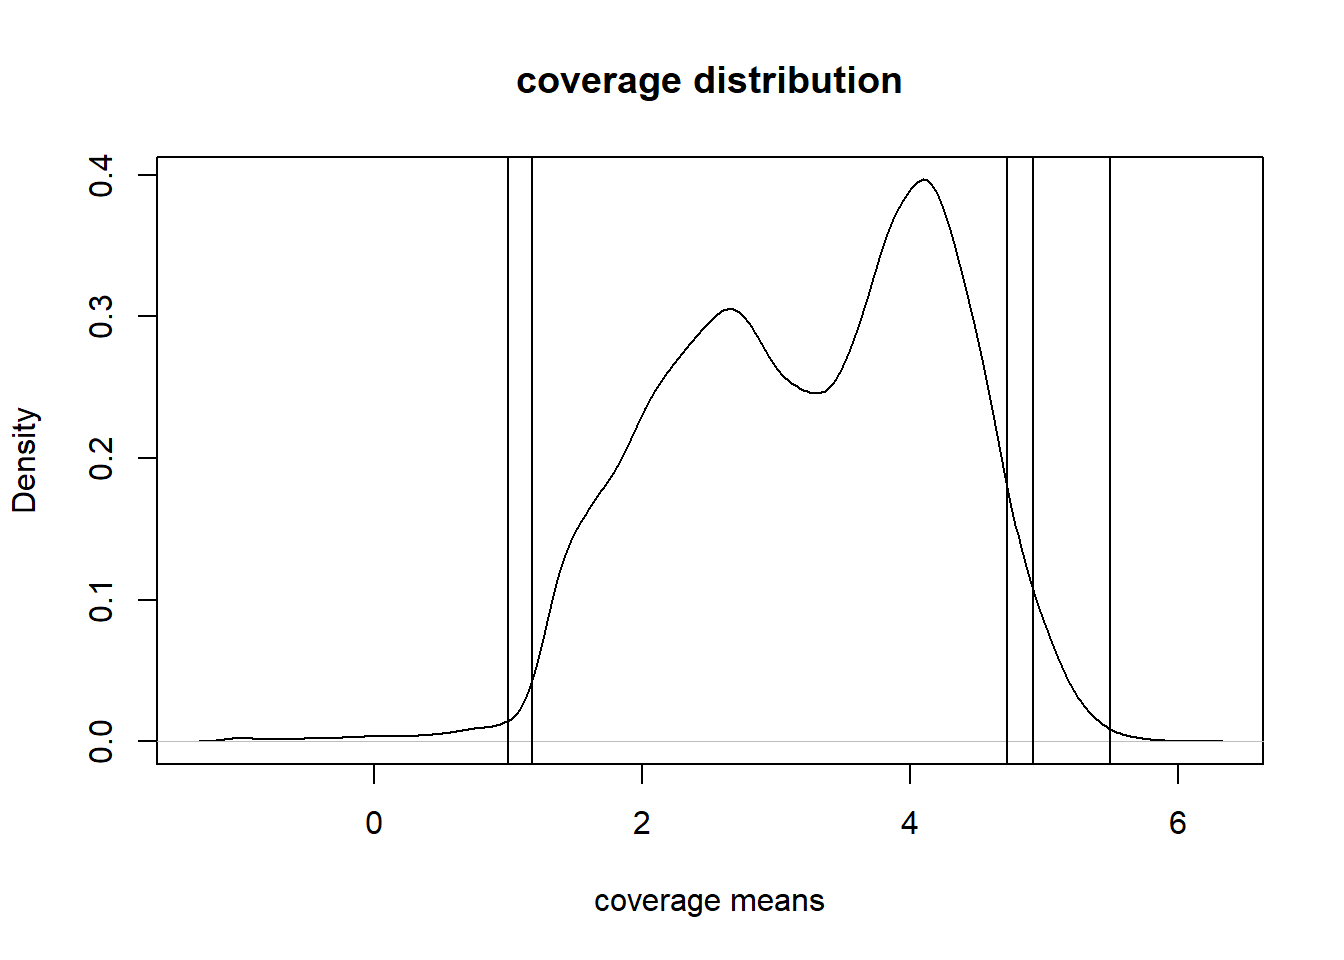
\includegraphics{Markdown_files/figure-latex/unnamed-chunk-7-1.pdf}

Both lower thresholds and the highest upper threshold seem to be fitting
looking at the diagram. But which threshold we will chose eventually
also depends on the percentage of deleted rows at the end of quality
control. We decided not to delete more than 15 \% of the rows, because
we don't want to risk to lose reliable information.

The procedure will now be used to set all the coverage values in
\texttt{cov\_genes} that are below or above the chosen threshold to NA.
Then all the beta-values associated to those NA coverage values are also
turned into NA. Eventually we will set another threshold for the
beta-values, defining the maximum number of NA that each row can have in
order not to be deleted. In order to do this, we used two nested
for-loops.

\paragraph{Preparing the first nested
for-loop}\label{preparing-the-first-nested-for-loop}

Before applying a threshold to the coverage values, the few \textbf{NAs
among the coverage values are set to 0} in order to allow the following
for loops to work. These values will be set to NAs again after the loop,
since 0 is below the lower threshold.

\begin{Shaded}
\begin{Highlighting}[]
\NormalTok{cov_genes[}\KeywordTok{is.na}\NormalTok{(cov_genes)] <-}\StringTok{ }\DecValTok{0}
\end{Highlighting}
\end{Shaded}

As the lower threshold we choose the coverage value 15, which is
positioned at a kink of the previously showed coverage distribution
diagram. As the upper coverage threshold we choose the 90 \% quantile.
Although it is not positioned at a kink in the diagram we consider it to
be a good threshold, because it still only leads to a removal of 7 \% of
the genes at the end of the quality control, which is far underneath the
chosen upper limit of 15 \%.

\begin{Shaded}
\begin{Highlighting}[]
\NormalTok{threshold1 <-}\StringTok{ }\DecValTok{15}
\NormalTok{threshold2 <-}\StringTok{ }\KeywordTok{quantile}\NormalTok{(cov_genes_means, }\DataTypeTok{probs =} \KeywordTok{seq}\NormalTok{(}\FloatTok{0.90}\NormalTok{,}\FloatTok{0.90}\NormalTok{,}\FloatTok{0.05}\NormalTok{))}
\end{Highlighting}
\end{Shaded}

\paragraph{The first nested for-loop}\label{the-first-nested-for-loop}

Now a \textbf{nested for-loop} is used to set the coverage values
underneath the lower threshold and above the upper threshold to NA. This
will be done for each row and each column of the dataframe
\texttt{cov\_genes}.

\begin{Shaded}
\begin{Highlighting}[]
\ControlFlowTok{for}\NormalTok{(i }\ControlFlowTok{in} \DecValTok{1}\OperatorTok{:}\KeywordTok{nrow}\NormalTok{(cov_genes))\{}
  \ControlFlowTok{for}\NormalTok{(j }\ControlFlowTok{in} \DecValTok{1}\OperatorTok{:}\KeywordTok{ncol}\NormalTok{(cov_genes))\{}
    \ControlFlowTok{if}\NormalTok{(}\KeywordTok{isTRUE}\NormalTok{(cov_genes[i,j] }\OperatorTok{<=}\StringTok{ }\NormalTok{threshold1))\{}
\NormalTok{      cov_genes[i,j] <-}\StringTok{ }\OtherTok{NA}
\NormalTok{    \} }
    \ControlFlowTok{if}\NormalTok{(}\KeywordTok{isTRUE}\NormalTok{(cov_genes[i,j] }\OperatorTok{>=}\StringTok{ }\NormalTok{threshold2))\{}
\NormalTok{      cov_genes[i,j] <-}\StringTok{ }\OtherTok{NA}
\NormalTok{    \}}
\NormalTok{  \}}
\NormalTok{\}}
\KeywordTok{rm}\NormalTok{(i,j,threshold1,threshold2)}
\end{Highlighting}
\end{Shaded}

\paragraph{Preparing the second nested
for-loop}\label{preparing-the-second-nested-for-loop}

A second nested for-loop is used to set the beta-values to NA that
correspond to the NA coverage values. A \textbf{dataframe containing
only beta-values} is created and the \textbf{genes located on the X- or
Y-chromosome are removed}.

\begin{Shaded}
\begin{Highlighting}[]
\NormalTok{beta_genes <-}\StringTok{ }\NormalTok{genes[,}\KeywordTok{c}\NormalTok{(}\DecValTok{1}\NormalTok{,}\DecValTok{11}\OperatorTok{:}\DecValTok{20}\NormalTok{)]}
\NormalTok{beta_genes_new <-}\StringTok{ }\NormalTok{beta_genes[}\OperatorTok{-}\KeywordTok{which}\NormalTok{(beta_genes }\OperatorTok{==}\StringTok{"chrX"}\NormalTok{),]}
\NormalTok{beta_genes <-}\StringTok{ }\NormalTok{beta_genes_new[}\OperatorTok{-}\KeywordTok{which}\NormalTok{(beta_genes_new }\OperatorTok{==}\StringTok{"chrY"}\NormalTok{),]}
\KeywordTok{rm}\NormalTok{(beta_genes_new)}
\NormalTok{beta_genes <-}\StringTok{ }\NormalTok{beta_genes [ ,}\KeywordTok{c}\NormalTok{(}\DecValTok{2}\OperatorTok{:}\DecValTok{11}\NormalTok{)]}
\end{Highlighting}
\end{Shaded}

\paragraph{The second nested for-loop}\label{the-second-nested-for-loop}

This \textbf{second nested for-loop} checks every row and every column
of the dataframe \texttt{cov\_genes}. If there is an NA, it sets the
belonging beta-value in \texttt{beta\_genes} to NA, too.

\begin{Shaded}
\begin{Highlighting}[]
\ControlFlowTok{for}\NormalTok{(k }\ControlFlowTok{in} \DecValTok{1}\OperatorTok{:}\KeywordTok{ncol}\NormalTok{(beta_genes))\{}
  \ControlFlowTok{for}\NormalTok{(l }\ControlFlowTok{in} \DecValTok{1}\OperatorTok{:}\KeywordTok{nrow}\NormalTok{(beta_genes))\{}
    \ControlFlowTok{if}\NormalTok{(}\KeywordTok{isTRUE}\NormalTok{(}\KeywordTok{is.na}\NormalTok{(cov_genes[k,l] }\OperatorTok{==}\StringTok{ }\OtherTok{TRUE}\NormalTok{)))\{}
\NormalTok{      beta_genes[k,l] <-}\StringTok{ }\OtherTok{NA}
\NormalTok{    \} }
\NormalTok{  \}}
\NormalTok{\}}
\KeywordTok{rm}\NormalTok{(k,l)}
\end{Highlighting}
\end{Shaded}

\paragraph{Finding a threshold for NAs among the
beta-values}\label{finding-a-threshold-for-nas-among-the-beta-values}

Now the second threshold in quality control needs to be chosen. The
threshold establishes how many NA are allowed per gene in order for the
gene not be completely deleted. Since some beta-values were set to NA in
the last step, we want to get insight in \textbf{how many NAs we
actually have now}.

\begin{Shaded}
\begin{Highlighting}[]
\NormalTok{rmv.rows_beta_genes =}\StringTok{ }\KeywordTok{apply}\NormalTok{(beta_genes,}\DecValTok{1}\NormalTok{, }\ControlFlowTok{function}\NormalTok{(x)\{}\KeywordTok{sum}\NormalTok{(}\KeywordTok{is.na}\NormalTok{(x))\})}
\end{Highlighting}
\end{Shaded}

A new dataframe containing only beta-values for genes which are below
the NA threshold is created. We chose a threshold of 3 allowed NAs per
row (gene), so \textbf{every row containing more than 3 NAs gets
removed}.

\begin{Shaded}
\begin{Highlighting}[]
\NormalTok{beta_genes_cleaned <-}\StringTok{ }\NormalTok{beta_genes[}\OperatorTok{-}\KeywordTok{which}\NormalTok{(rmv.rows_beta_genes }\OperatorTok{>}\DecValTok{2}\NormalTok{),]}
\end{Highlighting}
\end{Shaded}

To see \textbf{how many rows are deleted} due to quality control the
numer of rows before and after quality control is compared. We
additionally have a look at the \textbf{percantage of rows deleted} and
see whether it is beneath 15 \%.

\begin{Shaded}
\begin{Highlighting}[]
\NormalTok{row_difference =}\StringTok{ }\KeywordTok{nrow}\NormalTok{(genes)}\OperatorTok{-}\KeywordTok{nrow}\NormalTok{(beta_genes_cleaned)}
\KeywordTok{sum}\NormalTok{(row_difference)}
\end{Highlighting}
\end{Shaded}

\begin{verbatim}
## [1] 3915
\end{verbatim}

\begin{Shaded}
\begin{Highlighting}[]
\NormalTok{genes_deleted_percentage =}\StringTok{ }\NormalTok{row_difference}\OperatorTok{/}\KeywordTok{nrow}\NormalTok{(genes)}\OperatorTok{*}\DecValTok{100}
\KeywordTok{sum}\NormalTok{(genes_deleted_percentage)}
\end{Highlighting}
\end{Shaded}

\begin{verbatim}
## [1] 6.961856
\end{verbatim}

With 7\% we are beneath the recommended upper limit of 15 \% of deleted
rows.

\subsection{2) Normalisation}\label{normalisation}

The tidy beta-values we have now are an approximation of the percentage
of DNA-methylation. Biologically beta-values are easy to understand.
They range from 0 to 1, where 0 means unmethylated and 1 means fully
methylated. But their bounded range is also a disadvantage. It leads to
the problem that they can not be used for statistical tests like the
t-test, because they violate the Gaussian distribution. For highly
methylated gene regions and unmethylated gene regions beta-values are
very heteroscedastic, which means, that the variability of a variable is
unequal across the range of values. Therefore we have to normalise them.
Beta-values need to be transformed into M-values via a logit
transformation. M-values do not have a bounded range, they can be
infinite big and small. While the middle methylation range (beta-value
range of 0,2-0,8) is linear to M-values, outside this range the
beta-values are compressed and the M-values more accurate and
homoscedastic. This is why M-values can be used for statistical tests
and are absolutely necessary for further analysis.

\subsubsection{Preparing beta-values for logit
transformation}\label{preparing-beta-values-for-logit-transformation}

Logit transformation turns the extreme beta-values 0 and 1 into
-infinite and infinite. Further tests cannot be computed if some values
are equal to -infinite and infinite. Because of this, we \textbf{set 0
to a very small number higher than 0, and 1 to a very big number smaller
than 1}.

\begin{Shaded}
\begin{Highlighting}[]
\NormalTok{beta_genes_cleaned[beta_genes_cleaned}\OperatorTok{==}\DecValTok{0}\NormalTok{]<-}\FloatTok{0.00000001}
\NormalTok{beta_genes_cleaned[beta_genes_cleaned}\OperatorTok{==}\DecValTok{1}\NormalTok{]<-}\FloatTok{0.99999999}
\end{Highlighting}
\end{Shaded}

\paragraph{Creating two seperate data frames for sick and healthy
patients}\label{creating-two-seperate-data-frames-for-sick-and-healthy-patients}

In order to perform our normalisation, we \textbf{split our data into
beta-values of healthy and diseased patients.}

\begin{Shaded}
\begin{Highlighting}[]
\NormalTok{beta_genes_healthy <-}\StringTok{ }\NormalTok{beta_genes_cleaned[,}\KeywordTok{c}\NormalTok{(}\DecValTok{1}\OperatorTok{:}\DecValTok{5}\NormalTok{)]}
\NormalTok{beta_genes_cancer <-}\StringTok{ }\NormalTok{beta_genes_cleaned[,}\KeywordTok{c}\NormalTok{(}\DecValTok{6}\OperatorTok{:}\DecValTok{10}\NormalTok{)]}
\end{Highlighting}
\end{Shaded}

Now we are able to \textbf{replace the remaining NA's by the row means
of the different genes.}The rowmeans is different between healthy and
sick patients so it is important to work with the two separated
dataframes.

\begin{Shaded}
\begin{Highlighting}[]
\NormalTok{k <-}\StringTok{ }\KeywordTok{which}\NormalTok{(}\KeywordTok{is.na}\NormalTok{(beta_genes_healthy), }\DataTypeTok{arr.ind=}\OtherTok{TRUE}\NormalTok{)}
\NormalTok{beta_genes_healthy[k] <-}\StringTok{ }\KeywordTok{rowMeans}\NormalTok{(beta_genes_healthy, }\DataTypeTok{na.rm=}\OtherTok{TRUE}\NormalTok{)[k[,}\DecValTok{1}\NormalTok{]]}
\NormalTok{l <-}\StringTok{ }\KeywordTok{which}\NormalTok{(}\KeywordTok{is.na}\NormalTok{(beta_genes_cancer), }\DataTypeTok{arr.ind=}\OtherTok{TRUE}\NormalTok{)}
\NormalTok{beta_genes_cancer[l] <-}\StringTok{ }\KeywordTok{rowMeans}\NormalTok{(beta_genes_cancer, }\DataTypeTok{na.rm=}\OtherTok{TRUE}\NormalTok{)[l[,}\DecValTok{1}\NormalTok{]]}
\end{Highlighting}
\end{Shaded}

\subsubsection{Transforming beta-values into
M-values}\label{transforming-beta-values-into-m-values}

In the next step we \textbf{transform our beta-values into M-values} so
we are able to do statistical tests with the data. We calculate the
M-values with the following equation:

\[M-value = log2(beta-value/(1??? beta-value))\]

\begin{Shaded}
\begin{Highlighting}[]
\NormalTok{M_genes_healthy <-}\StringTok{ }\KeywordTok{log2}\NormalTok{(beta_genes_healthy}\OperatorTok{/}\NormalTok{(}\DecValTok{1}\OperatorTok{-}\NormalTok{(beta_genes_healthy)))}
\NormalTok{M_genes_cancer <-}\StringTok{ }\KeywordTok{log2}\NormalTok{(beta_genes_cancer}\OperatorTok{/}\NormalTok{(}\DecValTok{1}\OperatorTok{-}\NormalTok{(beta_genes_cancer)))}
\end{Highlighting}
\end{Shaded}

For applying the PCA on our data we have to build a \textbf{dataset
which contains sick and healthy patients} with \textbf{short column
names}.

\begin{Shaded}
\begin{Highlighting}[]
\NormalTok{M_genes <-}\StringTok{ }\KeywordTok{cbind}\NormalTok{(M_genes_healthy, M_genes_cancer)}
\KeywordTok{colnames}\NormalTok{(M_genes) <-}\StringTok{ }\KeywordTok{c}\NormalTok{(}\StringTok{"1H"}\NormalTok{,}\StringTok{"2H"}\NormalTok{,}\StringTok{"3H"}\NormalTok{,}\StringTok{"4H"}\NormalTok{,}\StringTok{"5H"}\NormalTok{,}\StringTok{"6CLL"}\NormalTok{,}\StringTok{"7CLL"}\NormalTok{,}\StringTok{"8CLL"}\NormalTok{,}\StringTok{"9CLL"}\NormalTok{,}\StringTok{"10CLL"}\NormalTok{)}
\end{Highlighting}
\end{Shaded}

\subsection{3) Dimensionality reduction}\label{dimensionality-reduction}

To \textbf{reduce our data} we use Principal Component Analysis. PCA
reduces a large set of variables into a smaller set which still contains
most information of the large dataset. Through the PCA, correlated
variables get transformed into a much smaller number of uncorrelated
variables which are called principal components. We want to have less
variables, because it is easier to work with them.

\subsubsection{PCA}\label{pca}

The code for the \textbf{PCA} expects the patients to be rows and the
samples to be columns. In our data the patients are columns and the
genes are rows so we have to \textbf{transpose the matrix} with the t()
function.

\begin{Shaded}
\begin{Highlighting}[]
\NormalTok{pca_M <-}\StringTok{ }\KeywordTok{prcomp}\NormalTok{(}\KeywordTok{t}\NormalTok{(M_genes))}
\end{Highlighting}
\end{Shaded}

\paragraph{How much variation does each component account
for?}\label{how-much-variation-does-each-component-account-for}

To decide, how much principal components we want to work with, we have
to know how much variation each principal component accounts for in
percentage. We plot the percentage for each component and decide with
the ``elbow method'' with which number of components we have to work
with.

\begin{Shaded}
\begin{Highlighting}[]
\NormalTok{var_pca <-}\StringTok{ }\NormalTok{pca_M}\OperatorTok{$}\NormalTok{sdev}\OperatorTok{^}\DecValTok{2}
\NormalTok{var_pca_per <-}\StringTok{ }\KeywordTok{round}\NormalTok{(var_pca}\OperatorTok{/}\KeywordTok{sum}\NormalTok{(var_pca)}\OperatorTok{*}\DecValTok{100}\NormalTok{, }\DecValTok{1}\NormalTok{)}
\KeywordTok{plot}\NormalTok{(var_pca_per, }\DataTypeTok{main=}\StringTok{"Variation of our data"}\NormalTok{, }\DataTypeTok{xlab=}\StringTok{"Principal Components"}\NormalTok{, }\DataTypeTok{ylab=}\StringTok{"Percent Variation"}\NormalTok{, }\DataTypeTok{ylim=}\KeywordTok{c}\NormalTok{(}\DecValTok{0}\NormalTok{,}\DecValTok{25}\NormalTok{),}\DataTypeTok{type =} \StringTok{"o"}\NormalTok{, }\DataTypeTok{pch=}\DecValTok{20}\NormalTok{)}
\end{Highlighting}
\end{Shaded}

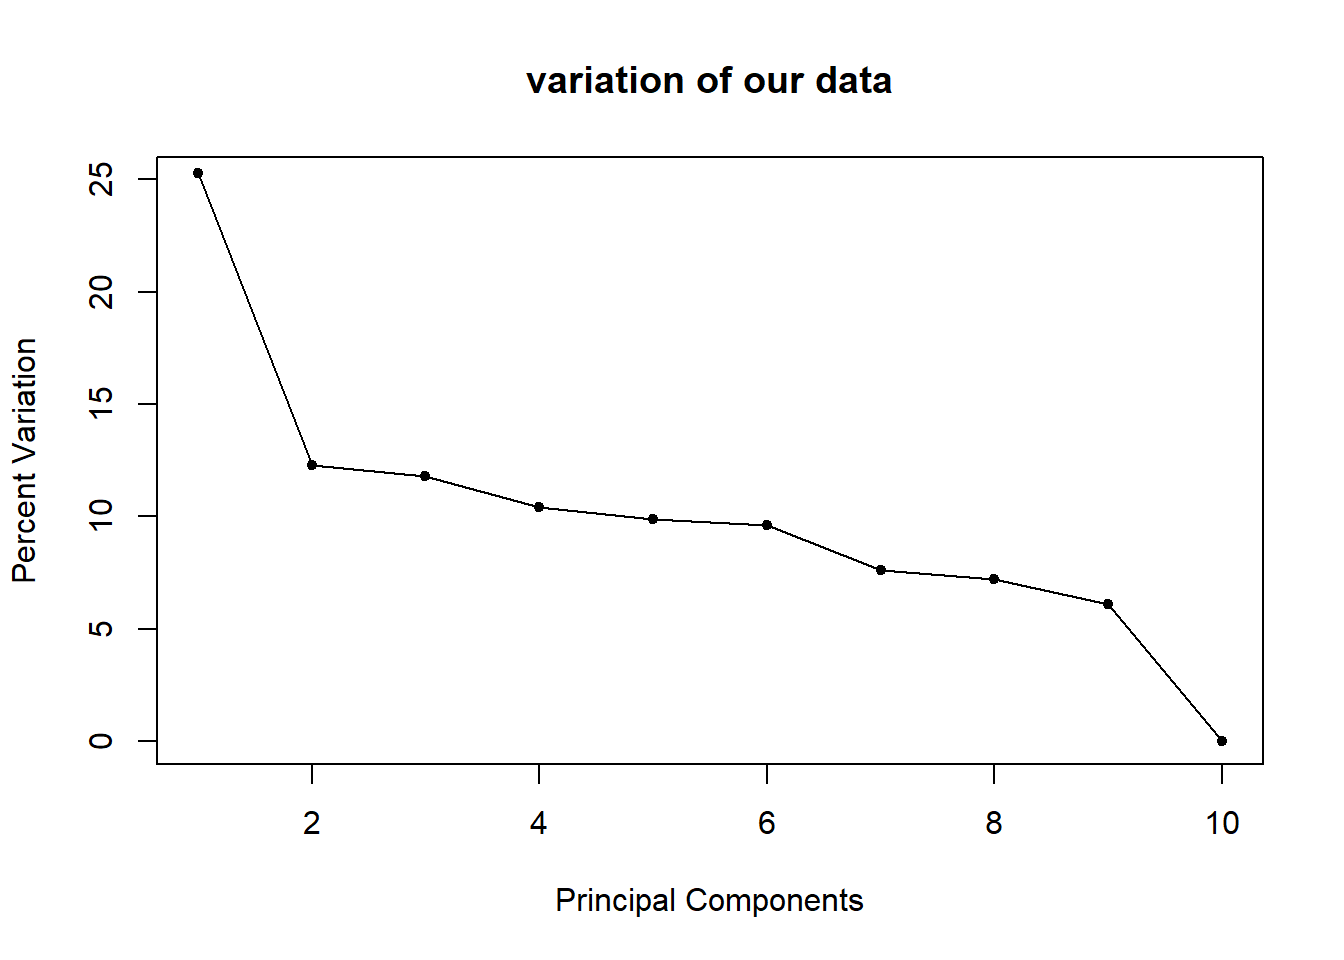
\includegraphics{Markdown_files/figure-latex/unnamed-chunk-22-1.pdf}

In the plot we can not see an elbow so we would actually have to work on
with ten principal components. But as the last PCs don't explain much
variation anyway and are therefor useless for us, we investigate on the
first five PCs.

\paragraph{Drawing a 2D plot of component 1 and
2}\label{drawing-a-2d-plot-of-component-1-and-2}

To check whether we have a batch effect, we plot principal component 1
against principle component 2.

\begin{Shaded}
\begin{Highlighting}[]
\KeywordTok{library}\NormalTok{(ggplot2)}
\end{Highlighting}
\end{Shaded}

\begin{verbatim}
## Warning: package 'ggplot2' was built under R version 3.5.2
\end{verbatim}

\begin{Shaded}
\begin{Highlighting}[]
\NormalTok{pca_values <-}\StringTok{ }\KeywordTok{data.frame}\NormalTok{(}\DataTypeTok{Sample=}\KeywordTok{rownames}\NormalTok{(pca_M}\OperatorTok{$}\NormalTok{x),}
                       \DataTypeTok{X=}\NormalTok{pca_M}\OperatorTok{$}\NormalTok{x[,}\DecValTok{1}\NormalTok{],}
                       \DataTypeTok{Y=}\NormalTok{pca_M}\OperatorTok{$}\NormalTok{x[,}\DecValTok{2}\NormalTok{])}
\KeywordTok{ggplot}\NormalTok{(}\DataTypeTok{data=}\NormalTok{pca_values, }\KeywordTok{aes}\NormalTok{(}\DataTypeTok{x=}\NormalTok{X, }\DataTypeTok{y=}\NormalTok{Y, }\DataTypeTok{label=}\NormalTok{Sample)) }\OperatorTok{+}
\StringTok{  }\KeywordTok{geom_text}\NormalTok{(}\KeywordTok{aes}\NormalTok{(}\DataTypeTok{colour =}\NormalTok{ annotation}\OperatorTok{$}\NormalTok{DISEASE)) }\OperatorTok{+}
\StringTok{  }\KeywordTok{xlab}\NormalTok{(}\KeywordTok{paste}\NormalTok{(}\StringTok{"PC1 - "}\NormalTok{, var_pca_per[}\DecValTok{1}\NormalTok{], }\StringTok{"%"}\NormalTok{, }\DataTypeTok{sep=}\StringTok{""}\NormalTok{)) }\OperatorTok{+}
\StringTok{  }\KeywordTok{ylab}\NormalTok{(}\KeywordTok{paste}\NormalTok{(}\StringTok{"PC2 - "}\NormalTok{, var_pca_per[}\DecValTok{2}\NormalTok{], }\StringTok{"%"}\NormalTok{, }\DataTypeTok{sep=}\StringTok{""}\NormalTok{)) }\OperatorTok{+}
\StringTok{  }\KeywordTok{theme_bw}\NormalTok{() }\OperatorTok{+}
\StringTok{  }\KeywordTok{ggtitle}\NormalTok{(}\StringTok{"PCA Graph of principal component 1 and 2"}\NormalTok{)}
\end{Highlighting}
\end{Shaded}

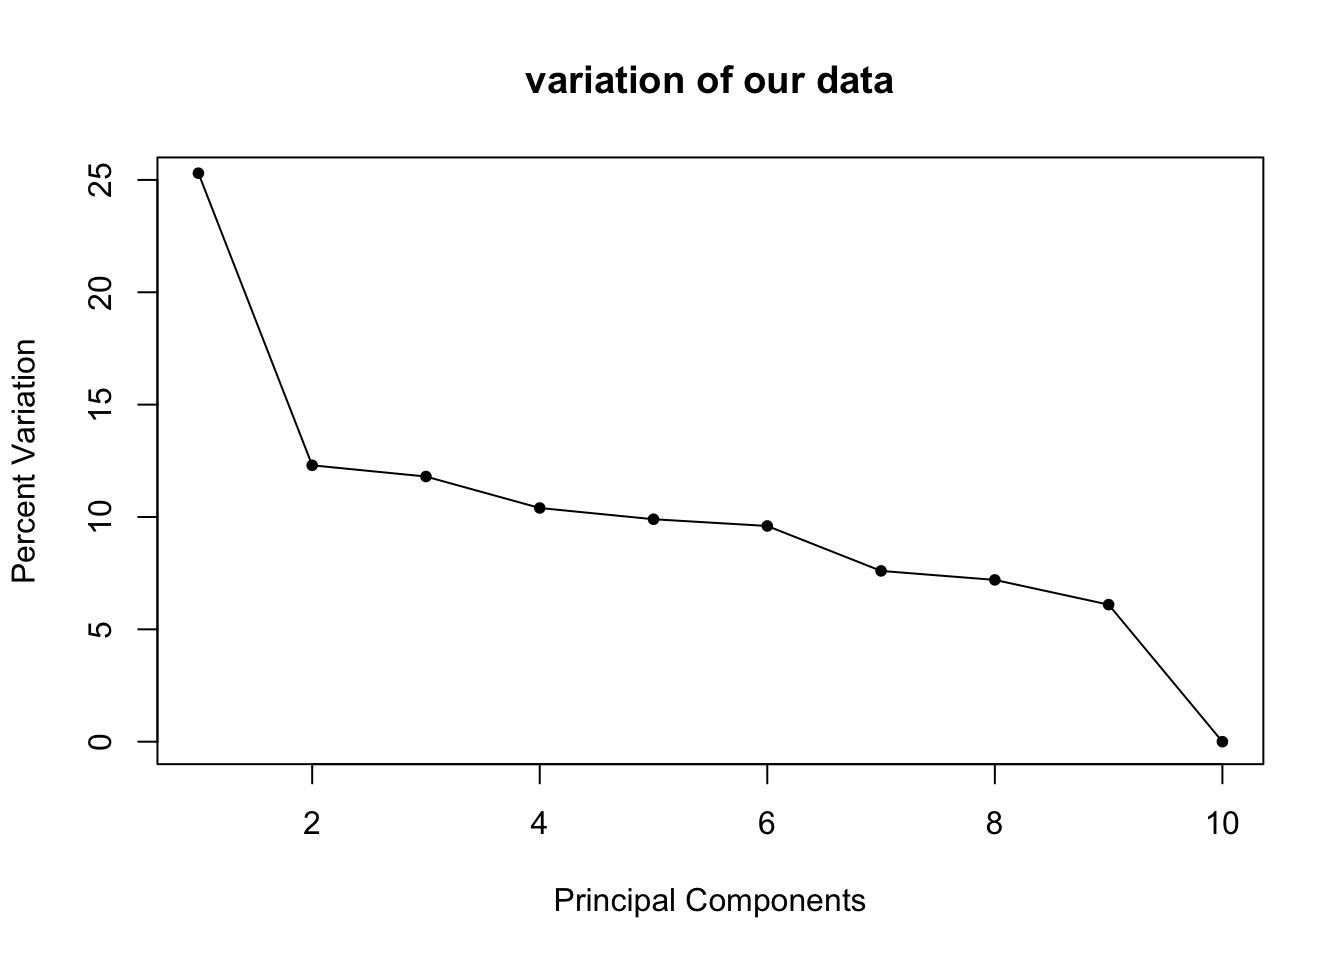
\includegraphics{Markdown_files/figure-latex/unnamed-chunk-23-1.pdf}

\subsubsection{Investigation for batch
effect}\label{investigation-for-batch-effect}

Now we use different categories of the annotation table which possibly
might cause \textbf{batch effect} and divide them by colour and shape in
our graph of principal component 1 and 2. Batch effect is a
\textbf{technical source of error}, which could have been added to the
samples by e.g.~gender. It is important that the technical variation
does not confound with the biology to not falsify the interpreted data.
To avoid errors, we used three tests to see whether there is a batch
effect in a principal component or not.

\begin{Shaded}
\begin{Highlighting}[]
\NormalTok{ggplot_}\DecValTok{1}\NormalTok{ <-}\StringTok{ }\KeywordTok{ggplot}\NormalTok{(}\DataTypeTok{data=}\NormalTok{pca_values, }\KeywordTok{aes}\NormalTok{(}\DataTypeTok{x=}\NormalTok{X, }\DataTypeTok{y=}\NormalTok{Y, }\DataTypeTok{label=}\NormalTok{Sample)) }\OperatorTok{+}
\StringTok{  }\KeywordTok{geom_point}\NormalTok{(}\KeywordTok{aes}\NormalTok{(}\DataTypeTok{shape=}\NormalTok{annotation}\OperatorTok{$}\NormalTok{cellTypeGroup, }\DataTypeTok{color=}\NormalTok{annotation}\OperatorTok{$}\NormalTok{Predicted.Gender)) }\OperatorTok{+}
\StringTok{  }\KeywordTok{xlab}\NormalTok{(}\KeywordTok{paste}\NormalTok{(}\StringTok{"PC1 - "}\NormalTok{, var_pca_per[}\DecValTok{1}\NormalTok{], }\StringTok{"%"}\NormalTok{, }\DataTypeTok{sep=}\StringTok{""}\NormalTok{)) }\OperatorTok{+}
\StringTok{  }\KeywordTok{ylab}\NormalTok{(}\KeywordTok{paste}\NormalTok{(}\StringTok{"PC2 - "}\NormalTok{, var_pca_per[}\DecValTok{2}\NormalTok{], }\StringTok{"%"}\NormalTok{, }\DataTypeTok{sep=}\StringTok{""}\NormalTok{)) }\OperatorTok{+}
\StringTok{  }\KeywordTok{theme_bw}\NormalTok{(}\DataTypeTok{base_size =} \DecValTok{6}\NormalTok{) }\OperatorTok{+}
\StringTok{  }\KeywordTok{ggtitle}\NormalTok{(}\StringTok{"PC1&2 check for gender"}\NormalTok{)}

\NormalTok{ggplot_}\DecValTok{2}\NormalTok{ <-}\StringTok{ }\KeywordTok{ggplot}\NormalTok{(}\DataTypeTok{data=}\NormalTok{pca_values, }\KeywordTok{aes}\NormalTok{(}\DataTypeTok{x=}\NormalTok{X, }\DataTypeTok{y=}\NormalTok{Y, }\DataTypeTok{label=}\NormalTok{Sample)) }\OperatorTok{+}
\StringTok{  }\KeywordTok{geom_point}\NormalTok{(}\KeywordTok{aes}\NormalTok{(}\DataTypeTok{shape=}\NormalTok{annotation}\OperatorTok{$}\NormalTok{cellTypeGroup, }\DataTypeTok{color=}\NormalTok{annotation}\OperatorTok{$}\NormalTok{SAMPLE_DESC_}\DecValTok{3}\NormalTok{)) }\OperatorTok{+}
\StringTok{  }\KeywordTok{xlab}\NormalTok{(}\KeywordTok{paste}\NormalTok{(}\StringTok{"PC1 - "}\NormalTok{, var_pca_per[}\DecValTok{1}\NormalTok{], }\StringTok{"%"}\NormalTok{, }\DataTypeTok{sep=}\StringTok{""}\NormalTok{)) }\OperatorTok{+}
\StringTok{  }\KeywordTok{ylab}\NormalTok{(}\KeywordTok{paste}\NormalTok{(}\StringTok{"PC2 - "}\NormalTok{, var_pca_per[}\DecValTok{2}\NormalTok{], }\StringTok{"%"}\NormalTok{, }\DataTypeTok{sep=}\StringTok{""}\NormalTok{)) }\OperatorTok{+}
\StringTok{  }\KeywordTok{theme_bw}\NormalTok{(}\DataTypeTok{base_size =} \DecValTok{6}\NormalTok{) }\OperatorTok{+}
\StringTok{  }\KeywordTok{ggtitle}\NormalTok{(}\StringTok{"PC1&2 check for cell type/origin"}\NormalTok{)}

\NormalTok{ggplot_}\DecValTok{4}\NormalTok{ <-}\StringTok{ }\KeywordTok{ggplot}\NormalTok{(}\DataTypeTok{data=}\NormalTok{pca_values, }\KeywordTok{aes}\NormalTok{(}\DataTypeTok{x=}\NormalTok{X, }\DataTypeTok{y=}\NormalTok{Y, }\DataTypeTok{label=}\NormalTok{Sample)) }\OperatorTok{+}
\StringTok{  }\KeywordTok{geom_point}\NormalTok{(}\KeywordTok{aes}\NormalTok{(}\DataTypeTok{shape=}\NormalTok{annotation}\OperatorTok{$}\NormalTok{cellTypeGroup, }\DataTypeTok{color=}\NormalTok{annotation}\OperatorTok{$}\NormalTok{DONOR_AGE)) }\OperatorTok{+}
\StringTok{  }\KeywordTok{xlab}\NormalTok{(}\KeywordTok{paste}\NormalTok{(}\StringTok{"PC1 - "}\NormalTok{, var_pca_per[}\DecValTok{1}\NormalTok{], }\StringTok{"%"}\NormalTok{, }\DataTypeTok{sep=}\StringTok{""}\NormalTok{)) }\OperatorTok{+}
\StringTok{  }\KeywordTok{ylab}\NormalTok{(}\KeywordTok{paste}\NormalTok{(}\StringTok{"PC2 - "}\NormalTok{, var_pca_per[}\DecValTok{2}\NormalTok{], }\StringTok{"%"}\NormalTok{, }\DataTypeTok{sep=}\StringTok{""}\NormalTok{)) }\OperatorTok{+}
\StringTok{  }\KeywordTok{theme_bw}\NormalTok{(}\DataTypeTok{base_size =} \DecValTok{6}\NormalTok{) }\OperatorTok{+}
\StringTok{  }\KeywordTok{ggtitle}\NormalTok{(}\StringTok{"PC1&2 check for age"}\NormalTok{)}

\NormalTok{ggplot_}\DecValTok{3}\NormalTok{ <-}\StringTok{ }\KeywordTok{ggplot}\NormalTok{(}\DataTypeTok{data=}\NormalTok{pca_values, }\KeywordTok{aes}\NormalTok{(}\DataTypeTok{x=}\NormalTok{X, }\DataTypeTok{y=}\NormalTok{Y, }\DataTypeTok{label=}\NormalTok{Sample)) }\OperatorTok{+}
\StringTok{  }\KeywordTok{geom_point}\NormalTok{(}\KeywordTok{aes}\NormalTok{(}\DataTypeTok{shape=}\NormalTok{annotation}\OperatorTok{$}\NormalTok{cellTypeGroup, }\DataTypeTok{color=}\NormalTok{annotation}\OperatorTok{$}\NormalTok{BIOMATERIAL_PROVIDER)) }\OperatorTok{+}
\StringTok{  }\KeywordTok{xlab}\NormalTok{(}\KeywordTok{paste}\NormalTok{(}\StringTok{"PC1 - "}\NormalTok{, var_pca_per[}\DecValTok{1}\NormalTok{], }\StringTok{"%"}\NormalTok{, }\DataTypeTok{sep=}\StringTok{""}\NormalTok{)) }\OperatorTok{+}
\StringTok{  }\KeywordTok{ylab}\NormalTok{(}\KeywordTok{paste}\NormalTok{(}\StringTok{"PC2 - "}\NormalTok{, var_pca_per[}\DecValTok{2}\NormalTok{], }\StringTok{"%"}\NormalTok{, }\DataTypeTok{sep=}\StringTok{""}\NormalTok{)) }\OperatorTok{+}
\StringTok{  }\KeywordTok{theme_bw}\NormalTok{(}\DataTypeTok{base_size =} \DecValTok{6}\NormalTok{) }\OperatorTok{+}
\StringTok{  }\KeywordTok{ggtitle}\NormalTok{(}\StringTok{"PC1&2 check for biomaterial provider"}\NormalTok{)}

\KeywordTok{library}\NormalTok{(gridExtra)}
\KeywordTok{library}\NormalTok{(ggplot2)}
\KeywordTok{grid.arrange}\NormalTok{(ggplot_}\DecValTok{1}\NormalTok{,ggplot_}\DecValTok{2}\NormalTok{, }\DataTypeTok{ncol=}\DecValTok{2}\NormalTok{)}
\end{Highlighting}
\end{Shaded}

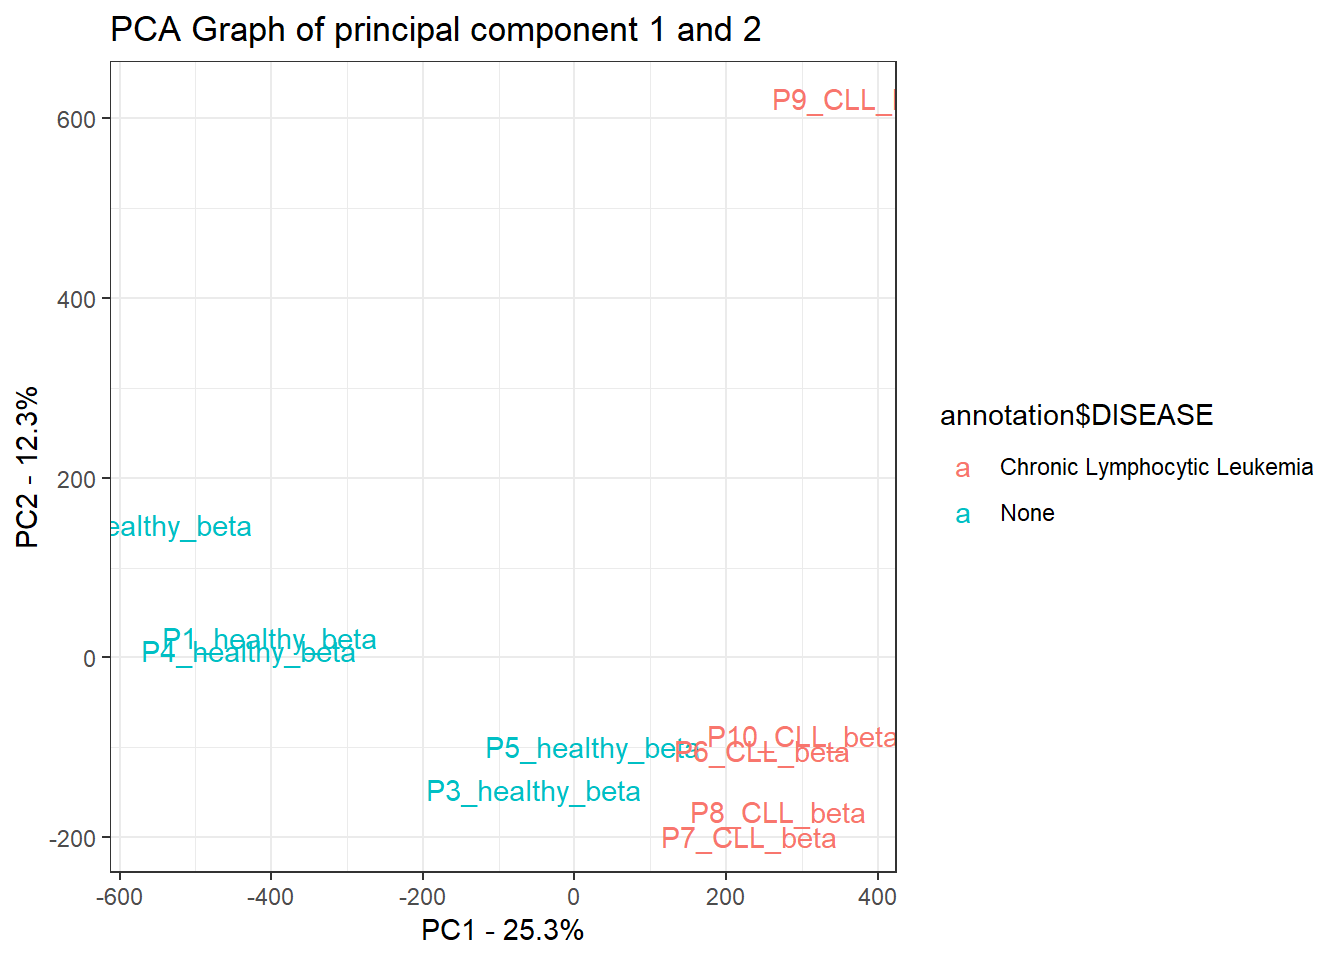
\includegraphics{Markdown_files/figure-latex/unnamed-chunk-24-1.pdf}

\begin{Shaded}
\begin{Highlighting}[]
\KeywordTok{grid.arrange}\NormalTok{(ggplot_}\DecValTok{3}\NormalTok{,ggplot_}\DecValTok{4}\NormalTok{, }\DataTypeTok{ncol=}\DecValTok{2}\NormalTok{)}
\end{Highlighting}
\end{Shaded}

\includegraphics{Markdown_files/figure-latex/unnamed-chunk-24-2.pdf}

\paragraph{Checking our PC 1 to 5 for significant batch effect per
category}\label{checking-our-pc-1-to-5-for-significant-batch-effect-per-category}

To verify our observations, we want to test if batch effect of the
different categories is significant for PC 1-5. Therefore, we first
create three dataframes containing PC 1-5 and the category of the
annotation table we want to investigate, depending on the properties of
the data, because we need to perform different tests for different data
types. For numbers we use the \textbf{permutation test} (of Pearson's r
correlation coefficient), for two categories the \textbf{Wilcoxon test}
and for more than two different categories the \textbf{Kruskal-Wallis
test}.

\begin{Shaded}
\begin{Highlighting}[]
\NormalTok{x <-}\StringTok{ }\NormalTok{pca_M[[}\StringTok{"x"}\NormalTok{]]}
\NormalTok{pca1_}\DecValTok{5}\NormalTok{ <-}\StringTok{ }\NormalTok{x[,}\DecValTok{1}\OperatorTok{:}\DecValTok{5}\NormalTok{]}
\NormalTok{batch_kruskal <-}\StringTok{ }\KeywordTok{data.frame}\NormalTok{(pca1_}\DecValTok{5}\NormalTok{, annotation}\OperatorTok{$}\NormalTok{SAMPLE_DESC_}\DecValTok{3}\NormalTok{)}
\NormalTok{batch_wilcoxon <-}\StringTok{ }\KeywordTok{data.frame}\NormalTok{(pca1_}\DecValTok{5}\NormalTok{, annotation}\OperatorTok{$}\NormalTok{BIOMATERIAL_PROVIDER, annotation}\OperatorTok{$}\NormalTok{DISEASE, annotation}\OperatorTok{$}\NormalTok{Predicted.Gender)}
\NormalTok{batch_permutation <-}\StringTok{ }\KeywordTok{data.frame}\NormalTok{ (pca1_}\DecValTok{5}\NormalTok{, annotation}\OperatorTok{$}\NormalTok{SEQ_RUNS_COUNT)}
\end{Highlighting}
\end{Shaded}

\paragraph{Permutation test for
numbers}\label{permutation-test-for-numbers}

The \textbf{permutation test} is a non-parametric test to check, whether
two not connected spot checks derive from the same basic total unit. The
H0 hypothesis assumes that both spot checks derive from the same basic
total unit. The permutation test in the usual form is tailored to the
counterhypothesis that the distributions of the two samples emerge by a
shift apart. Often the question is not only if there is a shift, but
also how big is this shift. Basically it is possible to check for a
batch effect with numbers.

\begin{Shaded}
\begin{Highlighting}[]
\NormalTok{cor.perm <-}\StringTok{ }\ControlFlowTok{function}\NormalTok{ (x, y, }\DataTypeTok{nperm =} \DecValTok{1000}\NormalTok{)}
\NormalTok{\{}
\NormalTok{  r.obs <-}\StringTok{ }\KeywordTok{cor}\NormalTok{ (}\DataTypeTok{x =}\NormalTok{ x, }\DataTypeTok{y =}\NormalTok{ y)}
\NormalTok{  P.par <-}\StringTok{ }\KeywordTok{cor.test}\NormalTok{ (}\DataTypeTok{x =}\NormalTok{ x, }\DataTypeTok{y =}\NormalTok{ y)}\OperatorTok{$}\NormalTok{p.value}
  \CommentTok{#  r.per <- replicate (nperm, expr = cor (x = x, y = sample (y)))}
\NormalTok{  r.per <-}\StringTok{ }\KeywordTok{sapply}\NormalTok{ (}\DecValTok{1}\OperatorTok{:}\NormalTok{nperm, }\DataTypeTok{FUN =} \ControlFlowTok{function}\NormalTok{ (i) }\KeywordTok{cor}\NormalTok{ (}\DataTypeTok{x =}\NormalTok{ x, }\DataTypeTok{y =} \KeywordTok{sample}\NormalTok{ (y)))}
\NormalTok{  r.per <-}\StringTok{ }\KeywordTok{c}\NormalTok{(r.per, r.obs)}
 
\NormalTok{  P.per <-}\StringTok{ }\KeywordTok{sum}\NormalTok{ (}\KeywordTok{abs}\NormalTok{ (r.per) }\OperatorTok{>=}\StringTok{ }\KeywordTok{abs}\NormalTok{ (r.obs))}\OperatorTok{/}\NormalTok{(nperm }\OperatorTok{+}\StringTok{ }\DecValTok{1}\NormalTok{) }
  \KeywordTok{return}\NormalTok{(}\KeywordTok{list}\NormalTok{(}\DataTypeTok{r.obs =}\NormalTok{ r.obs, }\DataTypeTok{P.par =}\NormalTok{ P.par, }\DataTypeTok{P.per =}\NormalTok{ P.per))}
\NormalTok{\}}

\NormalTok{x <-batch_permutation}\OperatorTok{$}\NormalTok{PC1}
\NormalTok{y <-batch_permutation}\OperatorTok{$}\NormalTok{annotation.SEQ_RUNS_COUNT}

\NormalTok{p_PC1_SEQ <-}\StringTok{ }\KeywordTok{cor.perm}\NormalTok{(x,y)}

\NormalTok{x <-batch_permutation}\OperatorTok{$}\NormalTok{PC2}
\NormalTok{p_PC2_SEQ <-}\StringTok{ }\KeywordTok{cor.perm}\NormalTok{(x,y)}

\NormalTok{x <-batch_permutation}\OperatorTok{$}\NormalTok{PC3}
\NormalTok{p_PC3_SEQ <-}\StringTok{ }\KeywordTok{cor.perm}\NormalTok{(x,y)}

\NormalTok{x <-batch_permutation}\OperatorTok{$}\NormalTok{PC4}
\NormalTok{p_PC4_SEQ <-}\StringTok{ }\KeywordTok{cor.perm}\NormalTok{(x,y)}

\NormalTok{x <-batch_permutation}\OperatorTok{$}\NormalTok{PC5}
\NormalTok{p_PC5_SEQ <-}\StringTok{ }\KeywordTok{cor.perm}\NormalTok{(x,y)}

\NormalTok{p_SEQ_RUNS_COUNT <-}\StringTok{ }\KeywordTok{data.frame}\NormalTok{(p_PC1_SEQ}\OperatorTok{$}\NormalTok{P.per, p_PC2_SEQ}\OperatorTok{$}\NormalTok{P.per, p_PC3_SEQ}\OperatorTok{$}\NormalTok{P.per, p_PC4_SEQ}\OperatorTok{$}\NormalTok{P.per, p_PC5_SEQ}\OperatorTok{$}\NormalTok{P.per)}
\end{Highlighting}
\end{Shaded}

\paragraph{Wilcoxon test for 2
categories}\label{wilcoxon-test-for-2-categories}

The \textbf{Wilcoxon test} for dependent spot checks tests, whether the
central tendencies are different. ``Dependent spot checks'' is used if
one measurement in a sample and one measurement in another sample
influence each other. In three situations this is the case: 1) Repeated
measures 2) Natural pairs 3) Matching Basically it is possible to check
for a batch effect with two categories only.

\begin{Shaded}
\begin{Highlighting}[]
\NormalTok{pc_1_BIOMATERIAL_PROVIDER <-}\StringTok{ }\KeywordTok{wilcox.test}\NormalTok{(batch_wilcoxon}\OperatorTok{$}\NormalTok{PC1 }\OperatorTok{~}\StringTok{ }\NormalTok{batch_wilcoxon}\OperatorTok{$}\NormalTok{annotation.BIOMATERIAL_PROVIDER, }\DataTypeTok{data =}\NormalTok{ batch_wilcoxon, }\DataTypeTok{exact =} \OtherTok{FALSE}\NormalTok{)}
\NormalTok{pc_2_BIOMATERIAL_PROVIDER <-}\StringTok{ }\KeywordTok{wilcox.test}\NormalTok{(batch_wilcoxon}\OperatorTok{$}\NormalTok{PC2 }\OperatorTok{~}\StringTok{ }\NormalTok{batch_wilcoxon}\OperatorTok{$}\NormalTok{annotation.BIOMATERIAL_PROVIDER, }\DataTypeTok{data =}\NormalTok{ batch_wilcoxon, }\DataTypeTok{exact =} \OtherTok{FALSE}\NormalTok{)}
\NormalTok{pc_3_BIOMATERIAL_PROVIDER <-}\StringTok{ }\KeywordTok{wilcox.test}\NormalTok{(batch_wilcoxon}\OperatorTok{$}\NormalTok{PC3 }\OperatorTok{~}\StringTok{ }\NormalTok{batch_wilcoxon}\OperatorTok{$}\NormalTok{annotation.BIOMATERIAL_PROVIDER, }\DataTypeTok{data =}\NormalTok{ batch_wilcoxon, }\DataTypeTok{exact =} \OtherTok{FALSE}\NormalTok{)}
\NormalTok{pc_4_BIOMATERIAL_PROVIDER <-}\StringTok{ }\KeywordTok{wilcox.test}\NormalTok{(batch_wilcoxon}\OperatorTok{$}\NormalTok{PC4 }\OperatorTok{~}\StringTok{ }\NormalTok{batch_wilcoxon}\OperatorTok{$}\NormalTok{annotation.BIOMATERIAL_PROVIDER, }\DataTypeTok{data =}\NormalTok{ batch_wilcoxon, }\DataTypeTok{exact =} \OtherTok{FALSE}\NormalTok{)}
\NormalTok{pc_5_BIOMATERIAL_PROVIDER <-}\StringTok{ }\KeywordTok{wilcox.test}\NormalTok{(batch_wilcoxon}\OperatorTok{$}\NormalTok{PC5 }\OperatorTok{~}\StringTok{ }\NormalTok{batch_wilcoxon}\OperatorTok{$}\NormalTok{annotation.BIOMATERIAL_PROVIDER, }\DataTypeTok{data =}\NormalTok{ batch_wilcoxon, }\DataTypeTok{exact =} \OtherTok{FALSE}\NormalTok{)}

\NormalTok{pc_1_BIOMATERIAL_PROVIDER <-}\StringTok{ }\NormalTok{pc_1_BIOMATERIAL_PROVIDER}\OperatorTok{$}\NormalTok{p.value}
\NormalTok{pc_2_BIOMATERIAL_PROVIDER <-}\StringTok{ }\NormalTok{pc_2_BIOMATERIAL_PROVIDER}\OperatorTok{$}\NormalTok{p.value}
\NormalTok{pc_3_BIOMATERIAL_PROVIDER <-}\StringTok{ }\NormalTok{pc_3_BIOMATERIAL_PROVIDER}\OperatorTok{$}\NormalTok{p.value}
\NormalTok{pc_4_BIOMATERIAL_PROVIDER <-}\StringTok{ }\NormalTok{pc_4_BIOMATERIAL_PROVIDER}\OperatorTok{$}\NormalTok{p.value}
\NormalTok{pc_5_BIOMATERIAL_PROVIDER <-}\StringTok{ }\NormalTok{pc_5_BIOMATERIAL_PROVIDER}\OperatorTok{$}\NormalTok{p.value}

\NormalTok{pc_1_DISEASE <-}\StringTok{ }\KeywordTok{wilcox.test}\NormalTok{(batch_wilcoxon}\OperatorTok{$}\NormalTok{PC1 }\OperatorTok{~}\StringTok{ }\NormalTok{batch_wilcoxon}\OperatorTok{$}\NormalTok{annotation.DISEASE, }\DataTypeTok{data =}\NormalTok{ batch_wilcoxon, }\DataTypeTok{exact =} \OtherTok{FALSE}\NormalTok{)}
\NormalTok{pc_2_DISEASE <-}\StringTok{ }\KeywordTok{wilcox.test}\NormalTok{(batch_wilcoxon}\OperatorTok{$}\NormalTok{PC2 }\OperatorTok{~}\StringTok{ }\NormalTok{batch_wilcoxon}\OperatorTok{$}\NormalTok{annotation.DISEASE, }\DataTypeTok{data =}\NormalTok{ batch_wilcoxon, }\DataTypeTok{exact =} \OtherTok{FALSE}\NormalTok{)}
\NormalTok{pc_3_DISEASE <-}\StringTok{ }\KeywordTok{wilcox.test}\NormalTok{(batch_wilcoxon}\OperatorTok{$}\NormalTok{PC3 }\OperatorTok{~}\StringTok{ }\NormalTok{batch_wilcoxon}\OperatorTok{$}\NormalTok{annotation.DISEASE, }\DataTypeTok{data =}\NormalTok{ batch_wilcoxon, }\DataTypeTok{exact =} \OtherTok{FALSE}\NormalTok{)}
\NormalTok{pc_4_DISEASE <-}\StringTok{ }\KeywordTok{wilcox.test}\NormalTok{(batch_wilcoxon}\OperatorTok{$}\NormalTok{PC4 }\OperatorTok{~}\StringTok{ }\NormalTok{batch_wilcoxon}\OperatorTok{$}\NormalTok{annotation.DISEASE, }\DataTypeTok{data =}\NormalTok{ batch_wilcoxon, }\DataTypeTok{exact =} \OtherTok{FALSE}\NormalTok{)}
\NormalTok{pc_5_DISEASE <-}\StringTok{ }\KeywordTok{wilcox.test}\NormalTok{(batch_wilcoxon}\OperatorTok{$}\NormalTok{PC5 }\OperatorTok{~}\StringTok{ }\NormalTok{batch_wilcoxon}\OperatorTok{$}\NormalTok{annotation.DISEASE, }\DataTypeTok{data =}\NormalTok{ batch_wilcoxon, }\DataTypeTok{exact =} \OtherTok{FALSE}\NormalTok{)}

\NormalTok{pc_1_DISEASE <-}\StringTok{ }\NormalTok{pc_1_DISEASE}\OperatorTok{$}\NormalTok{p.value}
\NormalTok{pc_2_DISEASE <-}\StringTok{ }\NormalTok{pc_2_DISEASE}\OperatorTok{$}\NormalTok{p.value}
\NormalTok{pc_3_DISEASE <-}\StringTok{ }\NormalTok{pc_3_DISEASE}\OperatorTok{$}\NormalTok{p.value}
\NormalTok{pc_4_DISEASE <-}\StringTok{ }\NormalTok{pc_4_DISEASE}\OperatorTok{$}\NormalTok{p.value}
\NormalTok{pc_5_DISEASE <-}\StringTok{ }\NormalTok{pc_5_DISEASE}\OperatorTok{$}\NormalTok{p.value}

\NormalTok{pc_1_Predicted.Gender <-}\StringTok{ }\KeywordTok{wilcox.test}\NormalTok{(batch_wilcoxon}\OperatorTok{$}\NormalTok{PC1 }\OperatorTok{~}\StringTok{ }\NormalTok{batch_wilcoxon}\OperatorTok{$}\NormalTok{annotation.Predicted.Gender, }\DataTypeTok{data =}\NormalTok{ batch_wilcoxon, }\DataTypeTok{exact =} \OtherTok{FALSE}\NormalTok{)}
\NormalTok{pc_2_Predicted.Gender <-}\StringTok{ }\KeywordTok{wilcox.test}\NormalTok{(batch_wilcoxon}\OperatorTok{$}\NormalTok{PC2 }\OperatorTok{~}\StringTok{ }\NormalTok{batch_wilcoxon}\OperatorTok{$}\NormalTok{annotation.Predicted.Gender, }\DataTypeTok{data =}\NormalTok{ batch_wilcoxon, }\DataTypeTok{exact =} \OtherTok{FALSE}\NormalTok{)}
\NormalTok{pc_3_Predicted.Gender <-}\StringTok{ }\KeywordTok{wilcox.test}\NormalTok{(batch_wilcoxon}\OperatorTok{$}\NormalTok{PC3 }\OperatorTok{~}\StringTok{ }\NormalTok{batch_wilcoxon}\OperatorTok{$}\NormalTok{annotation.Predicted.Gender, }\DataTypeTok{data =}\NormalTok{ batch_wilcoxon, }\DataTypeTok{exact =} \OtherTok{FALSE}\NormalTok{)}
\NormalTok{pc_4_Predicted.Gender <-}\StringTok{ }\KeywordTok{wilcox.test}\NormalTok{(batch_wilcoxon}\OperatorTok{$}\NormalTok{PC4 }\OperatorTok{~}\StringTok{ }\NormalTok{batch_wilcoxon}\OperatorTok{$}\NormalTok{annotation.Predicted.Gender, }\DataTypeTok{data =}\NormalTok{ batch_wilcoxon, }\DataTypeTok{exact =} \OtherTok{FALSE}\NormalTok{)}
\NormalTok{pc_5_Predicted.Gender <-}\StringTok{ }\KeywordTok{wilcox.test}\NormalTok{(batch_wilcoxon}\OperatorTok{$}\NormalTok{PC5 }\OperatorTok{~}\StringTok{ }\NormalTok{batch_wilcoxon}\OperatorTok{$}\NormalTok{annotation.Predicted.Gender, }\DataTypeTok{data =}\NormalTok{ batch_wilcoxon, }\DataTypeTok{exact =} \OtherTok{FALSE}\NormalTok{)}

\NormalTok{pc_1_Predicted.Gender <-}\StringTok{ }\NormalTok{pc_1_Predicted.Gender}\OperatorTok{$}\NormalTok{p.value}
\NormalTok{pc_2_Predicted.Gender <-}\StringTok{ }\NormalTok{pc_2_Predicted.Gender}\OperatorTok{$}\NormalTok{p.value}
\NormalTok{pc_3_Predicted.Gender <-}\StringTok{ }\NormalTok{pc_3_Predicted.Gender}\OperatorTok{$}\NormalTok{p.value}
\NormalTok{pc_4_Predicted.Gender <-}\StringTok{ }\NormalTok{pc_4_Predicted.Gender}\OperatorTok{$}\NormalTok{p.value}
\NormalTok{pc_5_Predicted.Gender <-}\StringTok{ }\NormalTok{pc_5_Predicted.Gender}\OperatorTok{$}\NormalTok{p.value}

\NormalTok{p_DISEASE <-}\StringTok{ }\KeywordTok{data.frame}\NormalTok{(pc_1_BIOMATERIAL_PROVIDER, pc_2_BIOMATERIAL_PROVIDER, pc_3_BIOMATERIAL_PROVIDER, pc_4_BIOMATERIAL_PROVIDER, pc_5_BIOMATERIAL_PROVIDER)}
\NormalTok{p_BIOMATERIAL_PROVIDER <-}\StringTok{ }\KeywordTok{data.frame}\NormalTok{(pc_1_BIOMATERIAL_PROVIDER, pc_2_BIOMATERIAL_PROVIDER, pc_3_BIOMATERIAL_PROVIDER, pc_4_BIOMATERIAL_PROVIDER, pc_5_BIOMATERIAL_PROVIDER)}
\NormalTok{p_Predicted.Gender <-}\StringTok{ }\KeywordTok{data.frame}\NormalTok{(pc_1_Predicted.Gender, pc_2_Predicted.Gender, pc_3_Predicted.Gender, pc_4_Predicted.Gender, pc_5_Predicted.Gender)}
\end{Highlighting}
\end{Shaded}

\paragraph{Kruskal-Wallis for several
categories}\label{kruskal-wallis-for-several-categories}

The \textbf{Kurskal-Wallis test} checks, whether there is a difference
in central tendencies between several independent spot checks. The test
is used, if the prerequisites for a parametric method is not fulfilled.
One of the benefits of the test is that the data does not have to be
normally distributed. On the other hand, the test can also be calculated
for small samples and outliers. Basically it is possible to check for a
batch effect with several categories.

\begin{Shaded}
\begin{Highlighting}[]
\NormalTok{batch_kruskal <-}\StringTok{ }\KeywordTok{within}\NormalTok{(batch_kruskal, \{}
\NormalTok{  PC1 <-}\StringTok{ }\KeywordTok{as.numeric}\NormalTok{(}\KeywordTok{as.character}\NormalTok{(PC1))}
\NormalTok{\})}

\NormalTok{batch_kruskal <-}\StringTok{ }\KeywordTok{within}\NormalTok{(batch_kruskal, \{}
\NormalTok{  PC2 <-}\StringTok{ }\KeywordTok{as.numeric}\NormalTok{(}\KeywordTok{as.character}\NormalTok{(PC2))}
\NormalTok{\})}

\NormalTok{batch_kruskal <-}\StringTok{ }\KeywordTok{within}\NormalTok{(batch_kruskal, \{}
\NormalTok{  PC3 <-}\StringTok{ }\KeywordTok{as.numeric}\NormalTok{(}\KeywordTok{as.character}\NormalTok{(PC3))}
\NormalTok{\})}

\NormalTok{batch_kruskal <-}\StringTok{ }\KeywordTok{within}\NormalTok{(batch_kruskal, \{}
\NormalTok{  PC4 <-}\StringTok{ }\KeywordTok{as.numeric}\NormalTok{(}\KeywordTok{as.character}\NormalTok{(PC4))}
\NormalTok{\})}

\NormalTok{batch_kruskal <-}\StringTok{ }\KeywordTok{within}\NormalTok{(batch_kruskal, \{}
\NormalTok{  PC5 <-}\StringTok{ }\KeywordTok{as.numeric}\NormalTok{(}\KeywordTok{as.character}\NormalTok{(PC5))}
\NormalTok{\})}

\NormalTok{sample_desc_3_pc1 <-}\StringTok{ }\KeywordTok{kruskal.test}\NormalTok{(batch_kruskal}\OperatorTok{$}\NormalTok{PC1 }\OperatorTok{~}\StringTok{ }\NormalTok{batch_kruskal}\OperatorTok{$}\NormalTok{annotation.SAMPLE_DESC_}\DecValTok{3}\NormalTok{, }\DataTypeTok{data =}\NormalTok{ batch_kruskal)}
\NormalTok{sample_desc_3_pc2 <-}\StringTok{ }\KeywordTok{kruskal.test}\NormalTok{(batch_kruskal}\OperatorTok{$}\NormalTok{PC2 }\OperatorTok{~}\StringTok{ }\NormalTok{batch_kruskal}\OperatorTok{$}\NormalTok{annotation.SAMPLE_DESC_}\DecValTok{3}\NormalTok{, }\DataTypeTok{data =}\NormalTok{ batch_kruskal)}
\NormalTok{sample_desc_3_pc3 <-}\StringTok{ }\KeywordTok{kruskal.test}\NormalTok{(batch_kruskal}\OperatorTok{$}\NormalTok{PC3 }\OperatorTok{~}\StringTok{ }\NormalTok{batch_kruskal}\OperatorTok{$}\NormalTok{annotation.SAMPLE_DESC_}\DecValTok{3}\NormalTok{, }\DataTypeTok{data =}\NormalTok{ batch_kruskal)}
\NormalTok{sample_desc_3_pc4 <-}\StringTok{ }\KeywordTok{kruskal.test}\NormalTok{(batch_kruskal}\OperatorTok{$}\NormalTok{PC4 }\OperatorTok{~}\StringTok{ }\NormalTok{batch_kruskal}\OperatorTok{$}\NormalTok{annotation.SAMPLE_DESC_}\DecValTok{3}\NormalTok{, }\DataTypeTok{data =}\NormalTok{ batch_kruskal)}
\NormalTok{sample_desc_3_pc5 <-}\StringTok{ }\KeywordTok{kruskal.test}\NormalTok{(batch_kruskal}\OperatorTok{$}\NormalTok{PC5 }\OperatorTok{~}\StringTok{ }\NormalTok{batch_kruskal}\OperatorTok{$}\NormalTok{annotation.SAMPLE_DESC_}\DecValTok{3}\NormalTok{, }\DataTypeTok{data =}\NormalTok{ batch_kruskal)}

\NormalTok{p_SAMPLE_DESC_}\DecValTok{3}\NormalTok{ <-}\StringTok{ }\KeywordTok{data.frame}\NormalTok{(sample_desc_3_pc1}\OperatorTok{$}\NormalTok{p.value, sample_desc_3_pc2}\OperatorTok{$}\NormalTok{p.value, sample_desc_3_pc3}\OperatorTok{$}\NormalTok{p.value, sample_desc_3_pc4}\OperatorTok{$}\NormalTok{p.value, sample_desc_3_pc5}\OperatorTok{$}\NormalTok{p.value)}
\end{Highlighting}
\end{Shaded}

We create a data frame containing \textbf{all p values of the
categories} we investigate for a batch effect.

\begin{Shaded}
\begin{Highlighting}[]
\NormalTok{p_DISEASE_t <-}\StringTok{ }\KeywordTok{as.data.frame}\NormalTok{(}\KeywordTok{t}\NormalTok{(p_DISEASE))}
\NormalTok{p_BIOMATERIAL_PROVIDER_t <-}\StringTok{ }\KeywordTok{as.data.frame}\NormalTok{(}\KeywordTok{t}\NormalTok{(p_BIOMATERIAL_PROVIDER))}
\NormalTok{p_Predicted.Gender_t <-}\StringTok{ }\KeywordTok{as.data.frame}\NormalTok{(}\KeywordTok{t}\NormalTok{(p_Predicted.Gender))}
\NormalTok{p_SEQ_RUNS_COUNT_t <-}\StringTok{ }\KeywordTok{as.data.frame}\NormalTok{(}\KeywordTok{t}\NormalTok{(p_SEQ_RUNS_COUNT))}
\NormalTok{p_SAMPLE_DESC_3_t <-}\StringTok{ }\KeywordTok{as.data.frame}\NormalTok{(}\KeywordTok{t}\NormalTok{( p_SAMPLE_DESC_}\DecValTok{3}\NormalTok{))}

\NormalTok{total_pvalue <-}\StringTok{ }\KeywordTok{cbind}\NormalTok{(p_DISEASE_t,p_BIOMATERIAL_PROVIDER_t,p_Predicted.Gender_t,p_SEQ_RUNS_COUNT_t,p_SAMPLE_DESC_3_t)}
\end{Highlighting}
\end{Shaded}

We give columns and rows informative names.

\begin{Shaded}
\begin{Highlighting}[]
\KeywordTok{names}\NormalTok{(total_pvalue)[}\DecValTok{1}\NormalTok{] <-}\StringTok{ "p_DISEASE"}
\KeywordTok{names}\NormalTok{(total_pvalue)[}\DecValTok{2}\NormalTok{] <-}\StringTok{ "p_BIOMATERIAL"}
\KeywordTok{names}\NormalTok{(total_pvalue)[}\DecValTok{3}\NormalTok{] <-}\StringTok{ "p_GENDER"}
\KeywordTok{names}\NormalTok{(total_pvalue)[}\DecValTok{4}\NormalTok{] <-}\StringTok{ "p_SEQ_RUNS_COUNT"}
\KeywordTok{names}\NormalTok{(total_pvalue)[}\DecValTok{5}\NormalTok{] <-}\StringTok{ "p_SAMPLE_DESC"}

\KeywordTok{rownames}\NormalTok{(total_pvalue)[}\KeywordTok{rownames}\NormalTok{(total_pvalue) }\OperatorTok{==}\StringTok{ "pc_1_BIOMATERIAL_PROVIDER"}\NormalTok{] <-}\StringTok{ "PC1"}
\KeywordTok{rownames}\NormalTok{(total_pvalue)[}\KeywordTok{rownames}\NormalTok{(total_pvalue) }\OperatorTok{==}\StringTok{ "pc_2_BIOMATERIAL_PROVIDER"}\NormalTok{] <-}\StringTok{ "PC2"}
\KeywordTok{rownames}\NormalTok{(total_pvalue)[}\KeywordTok{rownames}\NormalTok{(total_pvalue) }\OperatorTok{==}\StringTok{ "pc_3_BIOMATERIAL_PROVIDER"}\NormalTok{] <-}\StringTok{ "PC3"}
\KeywordTok{rownames}\NormalTok{(total_pvalue)[}\KeywordTok{rownames}\NormalTok{(total_pvalue) }\OperatorTok{==}\StringTok{ "pc_4_BIOMATERIAL_PROVIDER"}\NormalTok{] <-}\StringTok{ "PC4"}
\KeywordTok{rownames}\NormalTok{(total_pvalue)[}\KeywordTok{rownames}\NormalTok{(total_pvalue) }\OperatorTok{==}\StringTok{ "pc_5_BIOMATERIAL_PROVIDER"}\NormalTok{] <-}\StringTok{ "PC5"}
\end{Highlighting}
\end{Shaded}

\paragraph{Preparation for heatmap}\label{preparation-for-heatmap}

To \textbf{decide which PC we will use for further analysis}, we draw a
heatmap showing which principle component is affected significantly by a
batch effect. All significant p-values are shown in red and
non-significant ones in blue. For analyzing and comparing all p-values
we state all p-values under 0.1 as significant. To make visualization
easier we set values above the significance threshold to 10 and values
equal or below to 1, so we just have to find colours for 2 values.

\begin{Shaded}
\begin{Highlighting}[]
\NormalTok{total_pvalue <-}\StringTok{ }\KeywordTok{data.matrix}\NormalTok{(total_pvalue)}

\ControlFlowTok{for}\NormalTok{ (i }\ControlFlowTok{in} \DecValTok{1}\OperatorTok{:}\KeywordTok{ncol}\NormalTok{(total_pvalue))\{}
  \ControlFlowTok{for}\NormalTok{ (j }\ControlFlowTok{in} \DecValTok{1}\OperatorTok{:}\KeywordTok{nrow}\NormalTok{(total_pvalue))\{}
    \ControlFlowTok{if}\NormalTok{(}\KeywordTok{isTRUE}\NormalTok{(total_pvalue[i,j] }\OperatorTok{>}\StringTok{ }\FloatTok{0.1}\NormalTok{))\{}
\NormalTok{      total_pvalue[i,j] <-}\StringTok{ }\DecValTok{10}
\NormalTok{    \}}
    \ControlFlowTok{if}\NormalTok{ (}\KeywordTok{isTRUE}\NormalTok{(total_pvalue[i,j] }\OperatorTok{<=}\StringTok{ }\FloatTok{0.1}\NormalTok{))\{}
\NormalTok{      total_pvalue [i,j] <-}\StringTok{ }\DecValTok{1}
\NormalTok{    \}}
\NormalTok{  \}}
\NormalTok{\}}
\end{Highlighting}
\end{Shaded}

\paragraph{Heatmap}\label{heatmap}

\begin{Shaded}
\begin{Highlighting}[]
\KeywordTok{library}\NormalTok{(gplots)}
\end{Highlighting}
\end{Shaded}

\begin{verbatim}
## Warning: package 'gplots' was built under R version 3.5.2
\end{verbatim}

\begin{verbatim}
## 
## Attaching package: 'gplots'
\end{verbatim}

\begin{verbatim}
## The following object is masked from 'package:stats':
## 
##     lowess
\end{verbatim}

\begin{Shaded}
\begin{Highlighting}[]
\KeywordTok{par}\NormalTok{(}\DataTypeTok{cex.main =} \DecValTok{1}\NormalTok{)}
    
    \KeywordTok{heatmap.2}\NormalTok{(}
\NormalTok{      total_pvalue, }\DataTypeTok{main =} \StringTok{"Batch effect in our principal components"}\NormalTok{,}
      \KeywordTok{title}\NormalTok{(main, }\DataTypeTok{cex.main =} \DecValTok{1} \OperatorTok{*}\StringTok{ }\NormalTok{op[[}\StringTok{"cex.main"}\NormalTok{]]),}
      \DataTypeTok{margins =} \KeywordTok{c}\NormalTok{(}\DecValTok{8}\NormalTok{,}\DecValTok{5}\NormalTok{),}
      \DataTypeTok{Colv =} \OtherTok{NA}\NormalTok{, }
      \DataTypeTok{Rowv =} \OtherTok{NA}\NormalTok{,}
      \DataTypeTok{dendrogram =} \StringTok{"none"}\NormalTok{, }
      \DataTypeTok{sepwidth =} \KeywordTok{c}\NormalTok{(}\FloatTok{0.01}\NormalTok{, }\FloatTok{0.01}\NormalTok{), }
      \DataTypeTok{sepcolor =} \StringTok{"black"}\NormalTok{, }
      \DataTypeTok{trace=} \StringTok{"none"}\NormalTok{, }
      \DataTypeTok{col =} \KeywordTok{colorRampPalette}\NormalTok{(}\KeywordTok{c}\NormalTok{(}\StringTok{"salmon"}\NormalTok{,}\StringTok{"blue"}\NormalTok{)), }
      \DataTypeTok{breaks =} \KeywordTok{c}\NormalTok{(}\KeywordTok{seq}\NormalTok{(}\DecValTok{0}\NormalTok{, }\DecValTok{1}\NormalTok{, }\DataTypeTok{length =} \DecValTok{2}\NormalTok{),}
                 \KeywordTok{seq}\NormalTok{(}\FloatTok{1.1}\NormalTok{, }\DecValTok{10}\NormalTok{, }\DataTypeTok{length =} \DecValTok{2}\NormalTok{)),}
      \DataTypeTok{colsep =} \DecValTok{1}\OperatorTok{:}\KeywordTok{ncol}\NormalTok{(total_pvalue), }
      \DataTypeTok{rowsep =} \DecValTok{1}\OperatorTok{:}\KeywordTok{nrow}\NormalTok{(total_pvalue), }
      \DataTypeTok{cexCol =} \FloatTok{0.7}\NormalTok{,}
      \DataTypeTok{cexRow =} \DecValTok{1}\NormalTok{,}
      \DataTypeTok{key =} \OtherTok{FALSE}\NormalTok{)}
\end{Highlighting}
\end{Shaded}

\includegraphics{Markdown_files/figure-latex/unnamed-chunk-32-1.pdf}

By looking at the heatmap or at the p-values one can see that principal
component 1 has a batch effect. Therefore \textbf{we go on with our
analysis using principal component 2} which doesn't show a batch effect
at all.

\paragraph{create a dataframe with loading scores of the 10000 most
importat genes, which have the most influence for principal component
2.}\label{create-a-dataframe-with-loading-scores-of-the-10000-most-importat-genes-which-have-the-most-influence-for-principal-component-2.}

Now we want to \textbf{find the most important genes} which means that
we want to find the genes which have the most influence on the principal
component two. For that we use the loading scores which we can find in
rotation of the PCA. The loadings describe the weight of each gene in
the principal component. If a gene has a high loading it has a high
weight in the principal component. A loading can be positive or negative
but we will first have a look on the absolut values. We create a
dataframe containing the 2000 and 10000 most important genes in
principal component 2 in ranked order.

\begin{Shaded}
\begin{Highlighting}[]
\NormalTok{loading_scores <-}\StringTok{ }\NormalTok{pca_M}\OperatorTok{$}\NormalTok{rotation[,}\DecValTok{2}\NormalTok{]}
\NormalTok{gene_scores <-}\StringTok{ }\KeywordTok{abs}\NormalTok{(loading_scores) }
\NormalTok{ranked_gene_score <-}\StringTok{ }\KeywordTok{sort}\NormalTok{(gene_scores, }\DataTypeTok{decreasing=}\OtherTok{TRUE}\NormalTok{)}
\NormalTok{genes_top_}\DecValTok{10000}\NormalTok{ <-}\StringTok{ }\KeywordTok{names}\NormalTok{(ranked_gene_score[}\DecValTok{1}\OperatorTok{:}\DecValTok{10000}\NormalTok{])}
\NormalTok{genes_top_}\DecValTok{2000}\NormalTok{ <-}\StringTok{ }\KeywordTok{names}\NormalTok{(ranked_gene_score[}\DecValTok{1}\OperatorTok{:}\DecValTok{2000}\NormalTok{])}
\end{Highlighting}
\end{Shaded}

\paragraph{Look for elbow in top gene
variance}\label{look-for-elbow-in-top-gene-variance}

Now we want to \textbf{decide how many genes we want to keep for our
further analysis} by looking for an elbow in the plot of loading scores.

\begin{Shaded}
\begin{Highlighting}[]
\KeywordTok{plot}\NormalTok{(}\KeywordTok{abs}\NormalTok{(pca_M}\OperatorTok{$}\NormalTok{rotation[genes_top_}\DecValTok{10000}\NormalTok{,}\DecValTok{2}\NormalTok{]),}\DataTypeTok{type =} \StringTok{"o"}\NormalTok{, }\DataTypeTok{pch=}\DecValTok{20}\NormalTok{)}
\end{Highlighting}
\end{Shaded}

\includegraphics{Markdown_files/figure-latex/unnamed-chunk-34-1.pdf}

Actually there is a kink in the elbow plot of loading scores of the
genes at round about 2000 genes. K-means clustering already worked with
2000 genes but by using only 2000 genes we get only 3 significant
different methylated genes, which is not sufficient. By using 10000
genes we get 24 differentially methylated genes, which is an amount
which we can work with.

\subsection{4) Clustering with k-means}\label{clustering-with-k-means}

K-means is a method to find groups in the data. It uses an iterative
algorithm which means that there is a repitition of steps with the aim
of finding the right cluster for each datapoint. First step is the
clustering which means that the datapoints get split up into k clusters.
Each datapoint gets alloted to its next clusterpoint. Next step is an
updating of the clusters by calculating center of each cluster and
define them as new clusterpoints. These two steps will be repeated as
long as set in the code. By performing k-means clustering we want to
\textbf{check whether sick and healthy patients are separated in two
different clusters.} Therefor we first create two dataframes containing
all M-values from the 2000 and 10000 most important genes for principal
component 2.

\begin{Shaded}
\begin{Highlighting}[]
\NormalTok{k_means_data2 <-}\StringTok{ }\NormalTok{M_genes[genes_top_}\DecValTok{2000}\NormalTok{,]}
\NormalTok{k_means_data <-}\StringTok{ }\NormalTok{M_genes[genes_top_}\DecValTok{10000}\NormalTok{,]}

\NormalTok{k <-}\StringTok{ }\KeywordTok{kmeans}\NormalTok{(}\DataTypeTok{x =} \KeywordTok{t}\NormalTok{(k_means_data2), }\DataTypeTok{centers =} \DecValTok{2}\NormalTok{, }\DataTypeTok{iter.max =} \DecValTok{1000}\NormalTok{)}
\NormalTok{k <-}
\StringTok{  }\KeywordTok{kmeans}\NormalTok{(}
    \DataTypeTok{x =} \KeywordTok{t}\NormalTok{(k_means_data),}
    \DataTypeTok{centers =} \DecValTok{2}\NormalTok{,}
    \DataTypeTok{iter.max =} \DecValTok{1000}
\NormalTok{  )}

\NormalTok{cluster <-}\StringTok{ }\KeywordTok{data.frame}\NormalTok{(k[[}\StringTok{"cluster"}\NormalTok{]])}
\NormalTok{cluster}
\end{Highlighting}
\end{Shaded}

\begin{verbatim}
##       k...cluster...
## 1H                 2
## 2H                 2
## 3H                 1
## 4H                 2
## 5H                 1
## 6CLL               1
## 7CLL               1
## 8CLL               1
## 9CLL               1
## 10CLL              1
\end{verbatim}

One can see that our sick and healthy patients belong to two different
clusters so we can use principal component two for further testing.

\subsection{5) Identifying differetially methylated regions
(DMRs)}\label{identifying-differetially-methylated-regions-dmrs}

\subsubsection{Student's t-test}\label{students-t-test}

To see whether the methylation differences, so differences in M-values,
between the two Sample groups are significant, \textbf{a student t-test
is performed}. It can be used, because due to normalisation the
varaiance of the values are equal now. The test compares the mean
M-value of sick patients to the mean M-value of healthy patients and
gives a p-value, which is significant or not depending on how strict is
the threshold you set.

\begin{Shaded}
\begin{Highlighting}[]
\NormalTok{cluster <-}\StringTok{ }\NormalTok{k[[}\StringTok{"cluster"}\NormalTok{]]}
\NormalTok{p_value =}\StringTok{ }\OtherTok{NULL}
\ControlFlowTok{for}\NormalTok{(i }\ControlFlowTok{in} \DecValTok{1}\OperatorTok{:}\KeywordTok{nrow}\NormalTok{(k_means_data))\{}
\NormalTok{  x =}\StringTok{ }\NormalTok{k_means_data[i, }\DecValTok{1}\OperatorTok{:}\DecValTok{5}\NormalTok{]}
\NormalTok{  y =}\StringTok{ }\NormalTok{k_means_data[i, }\DecValTok{6}\OperatorTok{:}\DecValTok{10}\NormalTok{]}
\NormalTok{  t_test =}\StringTok{ }\KeywordTok{t.test}\NormalTok{(x, y)}
\NormalTok{  p_value[i] =}\StringTok{ }\NormalTok{t_test}\OperatorTok{$}\NormalTok{p.value}
\NormalTok{\}}
\end{Highlighting}
\end{Shaded}

We \textbf{create a dataframe wich contains the p-values} from t-test.

\begin{Shaded}
\begin{Highlighting}[]
\NormalTok{pvalues <-}\StringTok{ }\KeywordTok{data.frame}\NormalTok{(p_value)}
\end{Highlighting}
\end{Shaded}

To get the gene ID belonging to those p-values we \textbf{change the
rownames}.

\begin{Shaded}
\begin{Highlighting}[]
\NormalTok{row_names <-}\StringTok{ }\KeywordTok{row.names}\NormalTok{(k_means_data)}
\NormalTok{p_combined <-}\StringTok{ }\NormalTok{pvalues}
\KeywordTok{rownames}\NormalTok{(p_combined) <-}\StringTok{ }\NormalTok{row_names}
\end{Highlighting}
\end{Shaded}

\subsubsection{Correction of p values by using the holm
method}\label{correction-of-p-values-by-using-the-holm-method}

To reduce the family-wise error rate, which is the propability of
getting one ore more type 1 errors (also called false positive error),
the \emph{holm method} is used. Besides a \emph{dataframe} containing
the uncorrected p-values and the corrected p-values in rising order and
the belonging gene ID and symbol is created.

\begin{Shaded}
\begin{Highlighting}[]
\NormalTok{p_combined}\OperatorTok{$}\NormalTok{p_adjusted =}\StringTok{ }\KeywordTok{p.adjust}\NormalTok{(p_combined}\OperatorTok{$}\NormalTok{p_value, }\DataTypeTok{method =} \StringTok{"holm"}\NormalTok{)}
\NormalTok{p_holm <-}\StringTok{ }\KeywordTok{data.frame}\NormalTok{(p_combined)}
\NormalTok{symbols <-}\StringTok{ }\NormalTok{genes[}\KeywordTok{rownames}\NormalTok{(p_holm),]}
\NormalTok{holm <-}\StringTok{ }\KeywordTok{cbind}\NormalTok{(p_holm, }\StringTok{"Symbols"}\NormalTok{ =}\StringTok{ }\NormalTok{symbols}\OperatorTok{$}\NormalTok{symbol)}
\NormalTok{holm_new <-}\StringTok{ }\NormalTok{holm[}\KeywordTok{order}\NormalTok{(holm}\OperatorTok{$}\NormalTok{p_value),]}
\end{Highlighting}
\end{Shaded}

\subsubsection{Finding DMRs}\label{finding-dmrs}

\paragraph{Significant different methylated
genes}\label{significant-different-methylated-genes}

The p-values from the t-test were corrected with the holm method. 24
genes had a p-value under 0.1. Because of that we defined this genes of
healthy patients as significantly differently methylated than the ones
of sick patients. The most differently methylated gene is MIR-941-1. It
is a gene for a microRNA (non-coding and short RNA) that plays a role in
the transcriptional regulation of gene expression. MicroRNAs have an
influence on stability and translation of mRNAs by being a part of the
RNA induced silencing complex (RISC). RISC can bind mRNAs complementary
to its miRNA or siRNA. This can either inhibit or destabilize the mRNA,
so that less or no proteins coded by the mRNA get produced. MIR-941-1 is
known to be transcriptionally silenced in gastric cancer cells which
fits to our results. Other differently methylated genes in our dataset
which are coding for miRNAs were MIR3687-1, MIR1915, MIR8075, MIR941-2,
MIR941-3, MIR941-4 and MIR647. Another group of differently methylated
genes play a role in splicing. Three of the 24 tested genes coded for
the U6 subunit of the spliceosome, namely RNU6-481P, RNU6-638P and
RNU6-1237P. Splicing is part of the processing of the mRNA in eukaryotes
which makes it very important for the protein activity. Also, we found
out that RNU7-116P is differently methylated. RNU7-116P codes for a U7
small nuclear ribonucleoprotein which is used for histone RNA
processing. Both the U6 and U7 subunit both play a part in
transcriptional regulation. Due to this regulation, proteins can be
differently expressed which might lead to cancer development.

\paragraph{Genes we found in literature which are not significant
different
nethylated}\label{genes-we-found-in-literature-which-are-not-significant-different-nethylated}

Besides there have been genes, often correlated to CLL, which we found
in literature before. \textbf{Literature genes}, which we also found in
our initial dataset \texttt{genes} are those ones.

\begin{Shaded}
\begin{Highlighting}[]
\CommentTok{#grep("symbol", genes$symbol, value = TRUE)}
\end{Highlighting}
\end{Shaded}

\begin{itemize}
\tightlist
\item
  TWIST2
\item
  VHL
\item
  ABI3
\item
  ADORA3
\item
  PRF1
\item
  CLLU1
\item
  LPL
\item
  NOTCH1
\item
  SCARF1
\item
  TNF
\item
  CTBP2
\item
  EGR1
\end{itemize}

The following genes from the literature can be found in our dataset
heaped, as they probably belong to a family:

\begin{itemize}
\tightlist
\item
  NFAT
\item
  EBF
\item
  ODC
\end{itemize}

The \textbf{literature genes still existing in the dataframe after the
t-test} are those ones.

\begin{Shaded}
\begin{Highlighting}[]
\CommentTok{#grep("gene_name", holm_new$Symbols, value = TRUE)}
\end{Highlighting}
\end{Shaded}

\begin{itemize}
\tightlist
\item
  ENSG00000048462 -\textgreater{} TNFRSF17
\item
  ENSG00000159958 -\textgreater{} TNFRSF13C
\item
  ENSG00000232810 -\textgreater{} TNF
\item
  ENSG00000233125 -\textgreater{} ACTBP12 (Maybe not that important,
  because original gene out of literature was named ``CTBP2'')
\end{itemize}

Those ones still existing in the dataframe after the t-test and the 24
significant genes are the relevant genes which may have an impact on CLL
forming. We \textbf{create a dataframe of relevant genes} and their
p-valus to have an overview of genes we should do some research about.

\begin{Shaded}
\begin{Highlighting}[]
\NormalTok{relevant_genes1 <-}\StringTok{ }\NormalTok{holm_new[}\KeywordTok{c}\NormalTok{(}\DecValTok{1}\OperatorTok{:}\DecValTok{24}\NormalTok{),]}
\NormalTok{relevant_genes2 <-}\StringTok{ }\NormalTok{holm_new[}\KeywordTok{c}\NormalTok{(}\StringTok{"ENSG00000048462"}\NormalTok{,}\StringTok{"ENSG00000159958"}\NormalTok{,}\StringTok{"ENSG00000232810"}\NormalTok{,}\StringTok{"ENSG00000233125"}\NormalTok{),]}
\NormalTok{relevant_genes <-}\StringTok{ }\KeywordTok{rbind}\NormalTok{(relevant_genes1,relevant_genes2)}
\KeywordTok{print}\NormalTok{(relevant_genes)}
\end{Highlighting}
\end{Shaded}

\begin{verbatim}
##                      p_value   p_adjusted                    Symbols
## ENSG00000215946 1.175067e-09 1.175067e-05                   MIR941-1
## ENSG00000204802 1.015632e-08 1.015530e-04                       <NA>
## ENSG00000264890 1.376601e-08 1.376326e-04                       <NA>
## ENSG00000199643 1.475274e-08 1.474831e-04                   RNU4-90P
## ENSG00000206921 1.722710e-08 1.722021e-04                  RNU6-481P
## ENSG00000279920 2.285155e-08 2.284012e-04                       <NA>
## ENSG00000252391 3.152707e-08 3.150815e-04                  RNU6-638P
## ENSG00000277437 4.763914e-08 4.760580e-04                  MIR3687-1
## ENSG00000222071 6.322396e-08 6.317338e-04                    MIR1915
## ENSG00000273587 1.331822e-07 1.330624e-03                    SNORA78
## ENSG00000275908 1.661780e-07 1.660119e-03                       <NA>
## ENSG00000277942 2.189029e-07 2.186621e-03                    MIR8075
## ENSG00000207554 3.582260e-07 3.577961e-03                     MIR647
## ENSG00000211837 6.980247e-07 6.971173e-03                     TRAJ53
## ENSG00000278903 7.360642e-07 7.350337e-03                       <NA>
## ENSG00000273981 8.751361e-07 8.738234e-03                       <NA>
## ENSG00000274450 9.378005e-07 9.363000e-03                       <NA>
## ENSG00000216141 1.213785e-06 1.211721e-02 MIR941-2;MIR941-3;MIR941-4
## ENSG00000248979 3.518207e-06 3.511874e-02                  LAMTOR3P2
## ENSG00000278639 4.424737e-06 4.416330e-02                       <NA>
## ENSG00000258577 4.986456e-06 4.976483e-02                    SNRPGP1
## ENSG00000277532 5.631739e-06 5.619912e-02                       <NA>
## ENSG00000207508 9.249911e-06 9.229562e-02                 RNU6-1237P
## ENSG00000252749 9.339817e-06 9.318335e-02                  RNU7-116P
## ENSG00000048462 3.398150e-02 1.000000e+00                   TNFRSF17
## ENSG00000159958 9.172109e-02 1.000000e+00                  TNFRSF13C
## ENSG00000232810 2.391774e-01 1.000000e+00                        TNF
## ENSG00000233125 5.847920e-01 1.000000e+00                    ACTBP12
\end{verbatim}

\subsubsection{Some additional information to our genes out of the
literature}\label{some-additional-information-to-our-genes-out-of-the-literature}

\paragraph{Gene number one: ACTBP12}\label{gene-number-one-actbp12}

ACTBP12 is just a pseudogene with no specific function. As the gene out
of our literature analysis was named “CTBP2” and not “ACTBP12”,
this is not surprising. Still we wanted to see, whether there is a
relation between these genes.

\paragraph{Gene number two: TNF}\label{gene-number-two-tnf}

This gene belongs to the tumor necrosis factor (TNF) superfamily and
encodes a multifunctional proinflammatory cytokine. This cytokine is
mainly secreted by macrophages, which are also important for the immune
system. By binding to specific receptors, this cytokine is involved in
the regulation of a wide spectrum of biological processes including cell
proliferation, differentiation, apoptosis, lipid metabolism, and
coagulation. It is linked with a variety of diseases for example
autoimmune diseases but also cancer, which is important in our case.
These specific TNF receptors are expressed in a wide variety of tissues
in mammals, especially in leucocytes which include B-cells. This
signalling pathways, as already mentioned, is able to promote B-cell
survival and proliferation. Sources to TNF: (Rickert et al., 2011)
(Gravestein and Borst, 1998)

\paragraph{Gene number three:
TNFRSF13C}\label{gene-number-three-tnfrsf13c}

Tumor necrosis factor receptor superfamily member 13C (TNFRSF13C) is, as
the name suggests, a gene which encodes for a receptor of the TNF. It is
also known as B-cell-activating factor receptor (BAFF-R). In general,
BAFF promotes the proliferation and differentiation of B-cells.

Sources to TNFRSF13C: (Mackay et al., 2010)

\paragraph{Gene number four: TNFRSF17}\label{gene-number-four-tnfrsf17}

The protein encoded by the gene tumor necrosis factor receptor
superfamily member 17 (TNFRSF17) gene is a member of the TNF-receptor
superfamily. It is a receptor, especially expressed in mature B
lymphocytes and might play a role in B cell development. It leads to
NF-kappaB and MAPK8/JNK activation and therefore it binds to different
TRAF family members. It might transduce signals for cell survival and
proliferation.

Sources to TNFRSF17: RefSeq, Jul 2008

\paragraph{Sources in general:}\label{sources-in-general}

Gravestein, L.A., and Borst, J. (1998). Tumor necrosis factor receptor
family members in the immune system. Seminars in Immunology 10, 423-434.

Rickert, R.C., Jellusova, J., and Miletic, A.V. (2011). Signaling by the
tumor necrosis factor receptor superfamily in B-cell biology and
disease. Immunological reviews 244, 115-133.

Mackay, F., Figgett, W.A., Saulep, D., Lepage, M., and Hibbs, M.L.
(2010). B-cell stage and context-dependent requirements for survival
signals from BAFF and the B-cell receptor. Immunological reviews 237,
205-225.

RefSeq, Jul 2008

\subsubsection{Statistical and biological relevant methylation
differences in
genes}\label{statistical-and-biological-relevant-methylation-differences-in-genes}

A vulcano plot can help visualising whether a gene is claimed to be
differently methylated in healthy and sick patients because of
statistical reasons, which means a significant p-value or because of
biological reasons, which would be a big difference in the mean of the
M-values or beta-values. Only the genes which show both characteristics,
really have a significant methylation difference.

\paragraph{Fold change calculation}\label{fold-change-calculation}

On the x-axis of the volcano plot there is the \textbf{difference of the
beta-value means of each sample group}. This is the axis showing the
biological relevance. Usually for better visualization you use the log2
fold change of the M-values. Due to the negative M-values that exist,
this is mathematically not possible. Therefor we do not use the log2
fold change of the M-values, but the one of the beta-values.

\begin{Shaded}
\begin{Highlighting}[]
\NormalTok{beta_}\DecValTok{10000}\NormalTok{ <-}\StringTok{ }\NormalTok{beta_genes_cleaned[genes_top_}\DecValTok{10000}\NormalTok{,]}
\NormalTok{beta_10000_log <-}\StringTok{ }\KeywordTok{log2}\NormalTok{(beta_}\DecValTok{10000}\NormalTok{)}
\NormalTok{control <-}\StringTok{ }\NormalTok{beta_10000_log[, }\DecValTok{1}\OperatorTok{:}\DecValTok{5}\NormalTok{]}
\NormalTok{tumor <-}\StringTok{ }\NormalTok{beta_10000_log[, }\DecValTok{6}\OperatorTok{:}\DecValTok{10}\NormalTok{]}
\NormalTok{control_mean <-}\StringTok{ }\KeywordTok{apply}\NormalTok{(control, }\DecValTok{1}\NormalTok{, mean)}
\NormalTok{tumor_mean <-}\StringTok{ }\KeywordTok{apply}\NormalTok{(tumor, }\DecValTok{1}\NormalTok{, mean)}
\NormalTok{fold =}\StringTok{ }\NormalTok{control_mean }\OperatorTok{-}\StringTok{ }\NormalTok{tumor_mean}
\end{Highlighting}
\end{Shaded}

\paragraph{Visualisation including information about hyper- and
hypomethylation}\label{visualisation-including-information-about-hyper--and-hypomethylation}

Also on the y-axis we have to improvise: The y-axis shows the p-values
and therefor the statistical relevance. Actually the corrected p-values
should be used, but somehow a lot of p-values were corrected to the
value 1, which distorts the plot. Therefor we use the uncorrected
p-values for the y-axis and \textbf{create a volcano plot}

\begin{Shaded}
\begin{Highlighting}[]
\KeywordTok{plot}\NormalTok{(fold, }\OperatorTok{-}\KeywordTok{log10}\NormalTok{(p_value), }\DataTypeTok{ylim =} \KeywordTok{c}\NormalTok{(}\DecValTok{0}\NormalTok{,}\DecValTok{3}\NormalTok{))}
\end{Highlighting}
\end{Shaded}

\includegraphics{Markdown_files/figure-latex/unnamed-chunk-44-1.pdf}

To visualise genes that are statistically and biologically relevant and
subdivide them into upmethylated and hypomethylated genes in case of
cancer, we first \textbf{create thresholds for significance} in p-values
and beta-value-difference (fold).

\begin{Shaded}
\begin{Highlighting}[]
\NormalTok{threshold_significant =}\StringTok{ }\FloatTok{0.1}
\NormalTok{threshold_fold =}\StringTok{ }\FloatTok{0.05}
\end{Highlighting}
\end{Shaded}

We create a \textbf{filter for biological relevant genes} using the
threshold for beta-value-difference, one for \textbf{statistically
relevant genes} and one that \textbf{combines both in one filter}.

\begin{Shaded}
\begin{Highlighting}[]
\NormalTok{filter_by_fold =}\StringTok{ }\KeywordTok{abs}\NormalTok{(fold) }\OperatorTok{>=}\StringTok{ }\NormalTok{threshold_fold}
\NormalTok{filter_by_pvalue =}\StringTok{ }\KeywordTok{abs}\NormalTok{(p_value) }\OperatorTok{<=}\StringTok{ }\NormalTok{threshold_significant}
\NormalTok{filter_combined =}\StringTok{ }\NormalTok{filter_by_fold }\OperatorTok{&}\StringTok{ }\NormalTok{filter_by_pvalue}
\end{Highlighting}
\end{Shaded}

The genes which fit this filter and are \textbf{upmethylated} in cancer
cells are coloured in red, while the \textbf{hypomethylated} genes are
coloured in blue.

\begin{Shaded}
\begin{Highlighting}[]
\KeywordTok{plot}\NormalTok{(fold, }\OperatorTok{-}\KeywordTok{log10}\NormalTok{(p_value))}
\KeywordTok{points}\NormalTok{ (fold[filter_combined }\OperatorTok{&}\StringTok{ }\NormalTok{fold }\OperatorTok{<}\StringTok{ }\DecValTok{0}\NormalTok{],}
        \OperatorTok{-}\KeywordTok{log10}\NormalTok{(p_value[filter_combined }\OperatorTok{&}\StringTok{ }\NormalTok{fold }\OperatorTok{<}\StringTok{ }\DecValTok{0}\NormalTok{]),}
        \DataTypeTok{pch =} \DecValTok{16}\NormalTok{, }\DataTypeTok{col =} \StringTok{"red"}\NormalTok{)}

\KeywordTok{points}\NormalTok{ (fold[filter_combined }\OperatorTok{&}\StringTok{ }\NormalTok{fold }\OperatorTok{>}\StringTok{ }\DecValTok{0}\NormalTok{],}
        \OperatorTok{-}\KeywordTok{log10}\NormalTok{(p_value[filter_combined }\OperatorTok{&}\StringTok{ }\NormalTok{fold }\OperatorTok{>}\StringTok{ }\DecValTok{0}\NormalTok{]),}
        \DataTypeTok{pch =} \DecValTok{16}\NormalTok{, }\DataTypeTok{col =} \StringTok{"blue"}\NormalTok{)}
\end{Highlighting}
\end{Shaded}

\includegraphics{Markdown_files/figure-latex/unnamed-chunk-47-1.pdf}

\paragraph{Hyper- and hypomethylation in relevant
genes}\label{hyper--and-hypomethylation-in-relevant-genes}

We have had created a dataframe \texttt{relevant\_genes} containing the
genes which show significant differences in methylation and four genes,
which do not show significant methylation differences between sick and
healthy, but seem to be worth a look, because we read about them in
literature before. But to know wether those genes in cancer patients are
hyper or hypomethylated we need to have a look at the fold value.
Therefor we \textbf{add the fold values to the relevant genes}. Genes in
cancer patients are \textbf{upmethylated} if the \textbf{fold is
negative} and the absolute fold higher than 0.05. And Genes are
\textbf{downmethylated} if the \textbf{fold is positiv} and the absolute
fold higher than 0.05.

\begin{Shaded}
\begin{Highlighting}[]
\NormalTok{fold <-}\StringTok{ }\KeywordTok{data.frame}\NormalTok{(fold)}
\NormalTok{fold2 <-}\StringTok{ }\KeywordTok{as.data.frame}\NormalTok{(fold[}\KeywordTok{rownames}\NormalTok{(relevant_genes),])}
\NormalTok{relevant_genes <-}\StringTok{ }\KeywordTok{cbind}\NormalTok{(relevant_genes, }\StringTok{"fold"}\NormalTok{ =}\StringTok{ }\NormalTok{fold2}\OperatorTok{$}\NormalTok{fold)}
\KeywordTok{print}\NormalTok{(relevant_genes)}
\end{Highlighting}
\end{Shaded}

\begin{verbatim}
##                      p_value   p_adjusted                    Symbols
## ENSG00000215946 1.175067e-09 1.175067e-05                   MIR941-1
## ENSG00000204802 1.015632e-08 1.015530e-04                       <NA>
## ENSG00000264890 1.376601e-08 1.376326e-04                       <NA>
## ENSG00000199643 1.475274e-08 1.474831e-04                   RNU4-90P
## ENSG00000206921 1.722710e-08 1.722021e-04                  RNU6-481P
## ENSG00000279920 2.285155e-08 2.284012e-04                       <NA>
## ENSG00000252391 3.152707e-08 3.150815e-04                  RNU6-638P
## ENSG00000277437 4.763914e-08 4.760580e-04                  MIR3687-1
## ENSG00000222071 6.322396e-08 6.317338e-04                    MIR1915
## ENSG00000273587 1.331822e-07 1.330624e-03                    SNORA78
## ENSG00000275908 1.661780e-07 1.660119e-03                       <NA>
## ENSG00000277942 2.189029e-07 2.186621e-03                    MIR8075
## ENSG00000207554 3.582260e-07 3.577961e-03                     MIR647
## ENSG00000211837 6.980247e-07 6.971173e-03                     TRAJ53
## ENSG00000278903 7.360642e-07 7.350337e-03                       <NA>
## ENSG00000273981 8.751361e-07 8.738234e-03                       <NA>
## ENSG00000274450 9.378005e-07 9.363000e-03                       <NA>
## ENSG00000216141 1.213785e-06 1.211721e-02 MIR941-2;MIR941-3;MIR941-4
## ENSG00000248979 3.518207e-06 3.511874e-02                  LAMTOR3P2
## ENSG00000278639 4.424737e-06 4.416330e-02                       <NA>
## ENSG00000258577 4.986456e-06 4.976483e-02                    SNRPGP1
## ENSG00000277532 5.631739e-06 5.619912e-02                       <NA>
## ENSG00000207508 9.249911e-06 9.229562e-02                 RNU6-1237P
## ENSG00000252749 9.339817e-06 9.318335e-02                  RNU7-116P
## ENSG00000048462 3.398150e-02 1.000000e+00                   TNFRSF17
## ENSG00000159958 9.172109e-02 1.000000e+00                  TNFRSF13C
## ENSG00000232810 2.391774e-01 1.000000e+00                        TNF
## ENSG00000233125 5.847920e-01 1.000000e+00                    ACTBP12
##                         fold
## ENSG00000215946 -0.062098540
## ENSG00000204802          NaN
## ENSG00000264890 -0.087534616
## ENSG00000199643          NaN
## ENSG00000206921          NaN
## ENSG00000279920          NaN
## ENSG00000252391          NaN
## ENSG00000277437          NaN
## ENSG00000222071 17.415912725
## ENSG00000273587 16.170359452
## ENSG00000275908  0.056731496
## ENSG00000277942 -0.065590372
## ENSG00000207554 24.754040645
## ENSG00000211837          NaN
## ENSG00000278903          NaN
## ENSG00000273981          NaN
## ENSG00000274450          NaN
## ENSG00000216141 -0.113837067
## ENSG00000248979 -0.035460336
## ENSG00000278639 -0.122955439
## ENSG00000258577 -0.107881498
## ENSG00000277532          NaN
## ENSG00000207508  0.787502101
## ENSG00000252749          NaN
## ENSG00000048462  1.307070457
## ENSG00000159958 -1.316244737
## ENSG00000232810 -0.978602969
## ENSG00000233125 -0.006033483
\end{verbatim}

\subsection{6) Logistic regression}\label{logistic-regression}

Logistic regression is used to model the relationship between a binary
outcome variable and one or more predictor variables. In this case, the
predictor variables are methylation data of the genes and the outcome is
either healthy or sick. Hence we want to \textbf{predict a patient's
health status by the methylation status of their genes}.

We create a dataframe, which contains M values and health status of 7
random patients. Therefore, the M value dataframe needs to be
transformed first. We then add the patients' health status. This data
frame is used for generating the logistic regression model. We then do
cross validation by applying the regression model to the test set data
frame and by checking whether the predicted and actual health status
match, we can see if the regression model makes works.

\begin{Shaded}
\begin{Highlighting}[]
\NormalTok{log_regression <-}\StringTok{ }\NormalTok{k_means_data[,}\KeywordTok{c}\NormalTok{(}\DecValTok{1}\NormalTok{,}\DecValTok{2}\NormalTok{,}\DecValTok{4}\NormalTok{,}\DecValTok{5}\NormalTok{,}\DecValTok{8}\NormalTok{,}\DecValTok{9}\NormalTok{,}\DecValTok{10}\NormalTok{)]}
\NormalTok{log_regression <-}\StringTok{ }\KeywordTok{t}\NormalTok{(log_regression)}
\NormalTok{log_regression <-}\StringTok{ }\KeywordTok{data.frame}\NormalTok{(log_regression)}
\NormalTok{test_set <-}\StringTok{ }\NormalTok{k_means_data[,}\KeywordTok{c}\NormalTok{(}\DecValTok{3}\NormalTok{,}\DecValTok{6}\NormalTok{,}\DecValTok{7}\NormalTok{)]}
\NormalTok{test_set <-}\StringTok{ }\KeywordTok{data.frame}\NormalTok{(}\KeywordTok{t}\NormalTok{(test_set))}

\NormalTok{healthstatus <-}\StringTok{ }\NormalTok{annotation}\OperatorTok{$}\NormalTok{DISEASE}
\NormalTok{healthstatus <-}\StringTok{ }\KeywordTok{data.frame}\NormalTok{(healthstatus)}
\NormalTok{healthstatus_regression <-}\StringTok{ }\NormalTok{healthstatus[}\KeywordTok{c}\NormalTok{(}\DecValTok{1}\NormalTok{, }\DecValTok{2}\NormalTok{, }\DecValTok{4}\NormalTok{, }\DecValTok{5}\NormalTok{, }\DecValTok{8}\NormalTok{, }\DecValTok{9}\NormalTok{, }\DecValTok{10}\NormalTok{),]}

\NormalTok{train_set <-}\StringTok{ }\KeywordTok{cbind}\NormalTok{(healthstatus_regression, log_regression)}

\NormalTok{regression_model <-}\StringTok{ }\KeywordTok{glm}\NormalTok{(healthstatus_regression }\OperatorTok{~}\StringTok{ }\NormalTok{., }\DataTypeTok{family =} \StringTok{"binomial"}\NormalTok{, }\DataTypeTok{data =}\NormalTok{ train_set)}
\NormalTok{summary_regression_model <-}\StringTok{ }\KeywordTok{summary}\NormalTok{(regression_model)}
\NormalTok{summary_regression_model}\OperatorTok{$}\NormalTok{coefficients}
\end{Highlighting}
\end{Shaded}

\begin{verbatim}
##                    Estimate Std. Error       z value  Pr(>|z|)
## (Intercept)     -68.3042527  272581.35 -0.0002505830 0.9998001
## ENSG00000275217   4.6430226   17166.33  0.0002704727 0.9997842
## ENSG00000280145  25.3715551   98344.01  0.0002579878 0.9997942
## ENSG00000227979 -31.7522839  157443.93 -0.0002016736 0.9998391
## ENSG00000276242   2.3408763   14049.26  0.0001666192 0.9998671
## ENSG00000271650  -0.8263456   43984.03 -0.0000187874 0.9999850
## ENSG00000272312   1.4226377    4825.18  0.0002948362 0.9997648
\end{verbatim}

We only get estimate values for the genes shown above whereas the values
for the remainig genes are NA and therefore not shown in the table. This
is because of multicollinearity, which means that one or more predictor
variables are highly correlated and consequently do not contribute to
the regression model. The estimate value explains the influence of the
predictor variable on the outcome variable. Positive values indicate
that a gene contributes to health whereas genes with negative values
promote disease. It is notable that we get high standard errors, which
implies that the regression model is not very reliable. These high
standard error values result from mulitcollinearity.

\begin{Shaded}
\begin{Highlighting}[]
\NormalTok{prediction <-}\StringTok{ }\KeywordTok{predict}\NormalTok{(regression_model, }\DataTypeTok{newdata =}\NormalTok{ test_set, }\DataTypeTok{type =} \StringTok{"response"}\NormalTok{)}
\end{Highlighting}
\end{Shaded}

\begin{verbatim}
## Warning in predict.lm(object, newdata, se.fit, scale = 1, type =
## ifelse(type == : prediction from a rank-deficient fit may be misleading
\end{verbatim}

\begin{Shaded}
\begin{Highlighting}[]
\NormalTok{prediction}
\end{Highlighting}
\end{Shaded}

\begin{verbatim}
##           3H         6CLL         7CLL 
## 3.012131e-10 2.220446e-16 2.220446e-16
\end{verbatim}

\begin{Shaded}
\begin{Highlighting}[]
\KeywordTok{levels}\NormalTok{(train_set}\OperatorTok{$}\NormalTok{healthstatus_regression)}
\end{Highlighting}
\end{Shaded}

\begin{verbatim}
## [1] "Chronic Lymphocytic Leukemia" "None"
\end{verbatim}

Since we only have very few data available, the prediction of the
logistic regression model based on the train set containing 70\% of our
data does not correspond with the actual health status. Even though the
predicted probability is 10\^{}6 times higher for the healthy patient
than for the ones with CLL, it is still very close to 0, which implies
that the patient is probably sick. Therefore we use all data available
to model logistic regression without performing cross validation.

\begin{Shaded}
\begin{Highlighting}[]
\NormalTok{k_means_data_no_cv <-}\StringTok{ }\KeywordTok{t}\NormalTok{(k_means_data)}
\NormalTok{k_means_data_no_cv <-}\StringTok{ }\KeywordTok{data.frame}\NormalTok{(k_means_data_no_cv)}
\NormalTok{full_data <-}\StringTok{ }\KeywordTok{cbind}\NormalTok{(healthstatus, k_means_data_no_cv)}
\NormalTok{model_no_cv <-}\StringTok{ }\KeywordTok{glm}\NormalTok{(healthstatus }\OperatorTok{~}\StringTok{ }\NormalTok{., }\DataTypeTok{family =} \StringTok{"binomial"}\NormalTok{, }\DataTypeTok{data =}\NormalTok{ full_data)}
\NormalTok{prediction_no_cv <-}\StringTok{ }\KeywordTok{predict}\NormalTok{(model_no_cv, }\DataTypeTok{newdata =}\NormalTok{ full_data, }\DataTypeTok{type =} \StringTok{"response"}\NormalTok{)}
\end{Highlighting}
\end{Shaded}

\begin{verbatim}
## Warning in predict.lm(object, newdata, se.fit, scale = 1, type =
## ifelse(type == : prediction from a rank-deficient fit may be misleading
\end{verbatim}

\begin{Shaded}
\begin{Highlighting}[]
\NormalTok{summary_model_no_cv <-}\StringTok{ }\KeywordTok{summary}\NormalTok{(model_no_cv)}
\NormalTok{summary_model_no_cv}\OperatorTok{$}\NormalTok{coefficients}
\end{Highlighting}
\end{Shaded}

\begin{verbatim}
##                    Estimate Std. Error       z value  Pr(>|z|)
## (Intercept)     -62.3090250 123717.301 -5.036404e-04 0.9995982
## ENSG00000275217   5.0612636  10153.185  4.984902e-04 0.9996023
## ENSG00000280145  54.1513644 143983.605  3.760940e-04 0.9996999
## ENSG00000227979 -50.0417969 141092.708 -3.546732e-04 0.9997170
## ENSG00000276242   2.1658625   8097.999  2.674565e-04 0.9997866
## ENSG00000271650  -9.8198190  42406.585 -2.315635e-04 0.9998152
## ENSG00000272312  -0.3410775   7096.218 -4.806469e-05 0.9999616
## ENSG00000265127  -2.1800901   9128.043 -2.388343e-04 0.9998094
## ENSG00000271876   0.1846260   5218.514  3.537904e-05 0.9999718
## ENSG00000278927  -0.9134562   5588.323 -1.634580e-04 0.9998696
\end{verbatim}

We now apply the second model to our data set.

\begin{Shaded}
\begin{Highlighting}[]
\NormalTok{prediction_no_cv}
\end{Highlighting}
\end{Shaded}

\begin{verbatim}
##           1H           2H           3H           4H           5H 
## 1.000000e+00 1.000000e+00 1.000000e+00 1.000000e+00 1.000000e+00 
##         6CLL         7CLL         8CLL         9CLL        10CLL 
## 2.143345e-11 2.143345e-11 2.143345e-11 2.143345e-11 2.143345e-11
\end{verbatim}

The predicted probability to be healthy is 1 for the healthy patients
and very close to 0 for the sick patients, so it corresponds with the
actual health status. This is the result we expected, since we made the
prediction for the data we used to create the model.


\end{document}
